\documentclass{article}
% --- Korean translation support (xelatex + kotex) ---
\usepackage{kotex}
\usepackage{fontspec}
\setmainfont{NanumMyeongjo}[AutoFakeSlant=0.167]
\setsansfont{NanumGothic}[AutoFakeSlant=0.167]
\setmainhangulfont{NanumMyeongjo}[AutoFakeSlant=0.167]
\setsanshangulfont{NanumGothic}[AutoFakeSlant=0.167]
\setmonohangulfont{NanumGothicCoding}[AutoFakeSlant=0.167]
\setmonofont{NanumGothicCoding}[AutoFakeSlant=0.167]
\linespread{1.22}\selectfont
\renewcommand{\figurename}{그림}
\renewcommand{\tablename}{표}
\setlength{\parindent}{1.2em}
% --- end Korean support ---

\usepackage{microtype}
\usepackage{graphicx}
\usepackage{subfigure}
\usepackage{booktabs} %
\usepackage{enumitem}
\usepackage[dvipsnames]{xcolor}
\usepackage{listings}
\usepackage{lstautogobble}  %

\usepackage{hyperref}


\newcommand{\theHalgorithm}{\arabic{algorithm}}

\usepackage[accepted]{icml2026}

\usepackage{amsmath}
\usepackage{amssymb}
\usepackage{mathtools}
\mathtoolsset{showonlyrefs}
\usepackage{amsthm}
\usepackage{bm}
\usepackage{xspace}

\usepackage{mdframed}
\definecolor{theoremcolor}{rgb}{255, 255, 255}
\mdfsetup{
    backgroundcolor=theoremcolor,
    linewidth=1pt,
    leftline=true,
    topline=false,
    rightline=false,
    bottomline=false 
}

\newmdtheoremenv{definition}{Definition}
\newmdtheoremenv{proposition}{Proposition}
\newmdtheoremenv{corollary}{Corollary}
\newmdtheoremenv{theorem}{Theorem}
\newmdtheoremenv{lemma}{Lemma}
\newmdtheoremenv{example}{Example}


\def\h{{\bm{h}}}
\def\s{{\bm{s}}}
\def\x{{\bm{x}}}
\def\y{{\bm{y}}}
\def\z{{\bm{z}}}
\def\tauv{{\bm{\tau}}}

\def\RR{{\mathbb{R}}}
\def\NN{{\mathbb{N}}}
\def\EE{{\mathbb{E}}}
\def\PP{{\mathbb{P}}}

\def\cA{{\mathcal{A}}}
\def\cC{{\mathcal{C}}}
\def\cF{{\mathcal{F}}}
\def\cL{{\mathcal{L}}}
\def\cM{{\mathcal{M}}}
\def\cP{{\mathcal{P}}}
\def\cS{{\mathcal{S}}}
\def\cT{{\mathcal{T}}}
\def\cU{{\mathcal{U}}}
\def\cV{{\mathcal{V}}}
\def\cX{{\mathcal{X}}}
\def\cY{{\mathcal{Y}}}
\def\bcY{\boldsymbol{\mathcal{Y}}}

\newcommand{\Qsub}[1]{R_{#1}}
\newcommand{\Rsub}[1]{R_{#1}}

\def\arm{{\textsc{arm}}}
\def\ebm{{\textsc{ebm}}}
\def\lse{{\mathrm{LSE}}}
\def\softargmax{{\operatorname{softargmax}}}
\def\KL{{\mathrm{KL}}}
\def\ones{{\mathbf{1}}}

\def\len{{\mathrm{len}}}
\def\bos{\texttt{BOS}\xspace}
\def\eos{\texttt{EOS}\xspace}
\def\pad{\texttt{PAD}\xspace}
\def\voc{\cV}
\def\augvoc{\cA}

\def\iid{{i.i.d.\ }}
\def\aka{{a.k.a.\ }}
\def\wrt{{w.r.t.\ }}

\def\pref{p_{\mathrm{ref}}}
\def\piref{\pi_{\mathrm{ref}}}

\DeclareMathOperator*{\conv}{conv}
\DeclareMathOperator*{\dom}{dom}
\DeclareMathOperator*{\argmax}{argmax}
\DeclareMathOperator*{\argmin}{argmin}

\def\arsim{\overset{\text{AR}}{\sim}}

\definecolor{bluekeywords}{rgb}{0.13, 0.13, 1}
\definecolor{greencomments}{rgb}{0, 0.5, 0}
\definecolor{redstrings}{rgb}{0.9, 0, 0}
\definecolor{graynumbers}{rgb}{0.5, 0.5, 0.5}

\lstset{
    autogobble, columns=fullflexible, showspaces=false, showtabs=false,
    breaklines=true, showstringspaces=false, breakatwhitespace=true,
    escapeinside={(*@}{@*)}, commentstyle=\color{greencomments},
    keywordstyle=\color{bluekeywords}, stringstyle=\color{redstrings},
    numberstyle=\color{graynumbers}, basicstyle=\ttfamily\footnotesize, frame=l,
    framesep=12pt, xleftmargin=12pt, tabsize=4, captionpos=b }

    
\newcommand{\MB}[1]{\textcolor{magenta}{[MB: #1]}}
\newcommand{\GV}[1]{\textcolor{NavyBlue}{[GV: #1]}}
\newcommand{\VR}[1]{\textcolor{ForestGreen}{[VR: #1]}}
\newcommand{\MS}[1]{\textcolor{blue}{[MS: #1]}}
\newcommand{\TL}[1]{\textcolor{brown}{[TL: #1]}}
\newcommand{\green}[1]{\textcolor{ForestGreen}{#1}}

\usepackage[textsize=tiny]{todonotes}




\def\mytitle{Autoregressive Language Models는 은밀한 Energy-Based Models이다:\\
Next-Token Prediction의 Lookahead 능력에 대한 통찰}

\icmltitlerunning{Autoregressive Language Models are Secretly Energy-Based Models}

\begin{document}

\twocolumn[
\icmltitle{\mytitle}



\icmlsetsymbol{equal}{*}

\begin{icmlauthorlist}

\icmlauthor{Mathieu  Blondel}{gdm}
\icmlauthor{Michaël E. Sander}{gdm}
\icmlauthor{Germain Vivier-Ardisson}{gdm}
\icmlauthor{Tianlin Liu}{gdm}
\icmlauthor{Vincent Roulet}{gdm}

\end{icmlauthorlist}

\icmlaffiliation{gdm}{Google DeepMind}

\icmlcorrespondingauthor{}{mblondel@google.com}

\icmlkeywords{autoregressive models, energy-based model, maxent RL, dynamic programming}

\vskip 0.3in
]



\printAffiliationsAndNotice{}  %

\begin{abstract} 
자기회귀 모델(ARM)은 현재 지배적인 패러다임을 구성하고 있습니다.
대규모 언어 모델(LLM). 에너지 기반 모델(EBM)은 또 다른 클래스를 나타냅니다.
LLM 개발에서는 역사적으로 덜 널리 사용되었던 모델이지만 아직은
훈련 후 정렬에서 최적의 정책을 자연스럽게 특성화합니다. 이에
논문에서 우리는 이 두 가지 모델 클래스에 대한 통합된 관점을 제시합니다. 체인을 가져가는 중
확률의 법칙을 출발점으로 하여 명시적인 전단사를 확립합니다.
기능 공간에서 ARM과 EBM 사이는
최대 엔트로피 강화에서 소프트 벨만 방정식의 특수한 경우
학습.
이 전단론을 바탕으로 우리는
ARM 및 EBM의 지도 학습. 또한, 우리는
이론적 오류 한계를 제공하여 EBM을 ARM으로 증류합니다. 
우리의 결과는 ARM의 사전 계획 능력에 대한 통찰력을 제공합니다.
차세대 토큰 예측 패러다임을 기반으로 합니다.
 \end{abstract}

\section{Introduction}

다음 토큰 예측을 기반으로 하는 자동 회귀 모델(ARM)
패러다임은 현재 지배적인 접근법을 구성하고 있다.
대규모 언어 모델(LLM). 
그들의
주요 장점은 고도로 병렬화 가능한 훈련과 능력에 있습니다.
정확한 조상 샘플링을 수행합니다.
에너지 기반 모델(EBM)은 또 다른 종류의 모델을 나타냅니다.
본질적으로 앞을 내다볼 수 있는 능력이 있고,
시퀀스 수준을 정의하기 때문에
배포판. 그러나 역사적으로 이러한 현상은 덜 일반적이었습니다.
가능한 모든 집합에 대해 다루기 힘든 분할 함수를 계산해야 합니다.
시퀀스. 결과적으로, 그들은 훈련하고 훈련하는 것이 훨씬 더 어렵습니다.
종종 MCMC(Markov-chain Monte-Carlo) 방법이 필요합니다.

사전 훈련 후 LLM은 일반적으로 사후 훈련 정렬 단계를 거칩니다.
이 프로세스는 흔히 최대 엔트로피(MaxEnt) 강화로 구성됩니다.
학습(RL), \aka 엔트로피 정규화 RL, 여기서 확률을 구합니다.
기대되는 보상 간의 균형을 최대화하는 분배(또는 정책)
Kullback-Leibler(KL) 정규화 용어. 결정적으로, 우리가
가능한 모든 확률 분포의 집합, 이에 대한 분석 솔루션
이 목표는 바로 EBM입니다.
따라서 최대화하는 ARM을 찾는다.
이 목표는 동일합니다 
EBM을 ARM으로 증류하는 것입니다.

이러한 관점은 근본적인 질문을 제기합니다. ARM은 어느 정도까지 가능합니까?
대략적인 EBM?  확률적 그래픽 모델 관점에서 ARM은 다음과 같습니다.
베이지안 네트워크(방향성 그래픽 모델), EBM은 Markov 무작위임
필드(방향이 지정되지 않은 그래픽 모델).  그러나 ARM은 다음과 같은 체인 규칙을 따릅니다.
확률은 원칙적으로 모든 확률 분포를 분해할 수 있습니다.
ARM은 EBM으로 변환 가능해야 하며 그 반대의 경우도 마찬가지입니다.
이러한 직관을 바탕으로 통찰력을 제공하는 몇 가지 결과를 도출합니다.
ARM \wrt EBM의 근사력으로 결과적으로
다음 토큰 예측을 기반으로 함에도 불구하고 미리 계획할 수 있는 능력
패러다임.

\paragraph{Contributions.}

\begin{itemize}[topsep=0pt,itemsep=3pt,parsep=3pt,leftmargin=5pt]

\item ARM과 EBM의 통합된 뷰를 제공하여 명확한 구조를 보여줍니다.
    이 두 모델 클래스 간의 유사성.

\item 기능 공간(RL의 \aka 테이블 형식 설정)에서 우리는
    ARM과 EBM 사이의 정확한 전단사를 설정합니다(제안 \ref{prop:bijection}). 
    우리의 출발점이면서
    확률의 연쇄 법칙이므로 우리의 전단사(bijection)는 하나의 사례로 볼 수 있습니다
    MaxEnt RL의 소프트 벨만 방정식. 우리의 결과는
    우리의 설정
    소프트 벨만 방정식은 체인의 직접적인 결과로 자연스럽게 나타납니다.
    확률의 법칙.

\item 이 전단사를 바탕으로 우리는 등가성을 도출합니다.
    ARM과 EBM의 지도 학습 사이(제안 \ref{prop:same_minima}). 게다가 우리는
    EBM을 ARM으로 추출하기 위한 오류 범위를 도출합니다(제안 \ref{prop:kl_bound}). 
    MaxEnt RL과 동일한 프로세스입니다. 
    수치 실험을 통해 검증된 우리의 결과는
    다음 토큰 예측에 대한 이론적 근거를 제공합니다.
    패러다임과 교사 강요.

\end{itemize}

\paragraph{Notation.}

$V$를 어휘 크기로 두고 $\voc \coloneqq \{1, \ldots, V\}$를
어휘 세트.  우리는 어휘에서 $t$ 크기의 시퀀스 집합을 다음과 같이 나타냅니다.
 $\voc^t$ .  $\voc$에서 제외된 두 가지 특수 토큰인 \bos를 고려합니다. 
(시퀀스의 시작) 프롬프트의 시작과 \eos를 인코딩하는 토큰 
(시퀀스 끝) 응답의 끝을 인코딩하는 토큰입니다.
그런 다음 최대 크기 $U$(\bos 포함)의 프롬프트 세트를 $\cX =
\{\bos\} \times \cup_{t=1}^{U-1} \voc^t$로 표시합니다.
최대 크기 $T$(\eos 포함)의 응답 세트 
 $\cY = \cup_{t=1}^{T-1} \voc^t \times \{\eos\}$ . 
$\y = (y_1, \dots, y_\tau) \in \cY$ 응답은 항상 \eos로 끝납니다.
 $y_\tau = \eos$ .  $\y$ ($\eos$ 포함)의 길이를 $|\y|$ 로 나타냅니다.
$t > 1$를 $\y_{<t} \coloneqq (y_1, \cdots, y_{t-1})$로 표시하고
우리는 $\y_{<1} \coloneqq \varnothing $를 설정했습니다. 우리는 다음과 같이 보강된 어휘를 나타냅니다.
\eos 토큰은 $\augvoc \coloneqq \cV \cup \{\eos\}$ 입니다.  우리는 $\oplus$를 사용하여
연결을 나타냅니다.  확률 변수를 대문자로 표시합니다. 예:
 $Y$ .  유한 집합 $\cY$가 주어지면 확률 공간을 정의합니다.
$\cY$에 대한 \textit{with full support} 분포를 $\cP(\cY)$로 하고
$f \colon \cY \to \RR$를 $\cF(\cY)$로 기능합니다.  $f \in
\cF(\cY)$ 함수가 주어지면 $\softargmax(f) \in \cP(\cY)$를 $\softargmax(f)(\y)
\coloneqq \frac{\exp f(\y)}{ \sum_{\y' \in \cY} \exp f(\y')}$로 정의합니다.

\section{A unified perspective on EBMs and ARMs} 
 \label{sec:unified_perspective}

\subsection{Energy-based models (EBMs)}

\paragraph{Model definition.}

EBM \citep{ackley1985learning,lecun2006tutorial}는 $R \colon \cX
\times \cY \to \RR$ 함수를 사용합니다.
입력 $\x \in \cX$ 사이의 '친화도' 측정(프롬프트) 
및 출력 $\y \in \cY$(완전한 응답).
우리는 값이 높을수록 선호도가 높다는 관례를 사용합니다.
따라서 $R$는 부정적인 에너지로 해석될 수 있습니다.
EBM은 다음과 같이 정의됩니다.
 \begin{equation} 
p^ \ebm _R( \y | \x ) 
 \coloneqq \frac{\exp(R(\x, \y))} { \sum _{ \y ' \in \cY } \exp (R( \x , \y '))},
 \label{eq:ebm_def} 
 \end{equation} 
혹은 좀 더 간략하게 말하면,
 $p^\ebm_R(\cdot|\x) = \mathrm{softargmax}(R(\x, \cdot))$ .
우리는 보상의 개념과 일치하기 때문에 의도적으로 $R$ 문자를 사용합니다.
RL의 기능.  보상은 학습된 모델이거나 주어진 기능일 수 있습니다.
검증인으로서.

연관된 시퀀스 수준 로그 파티션 기능은 다음과 같습니다.
 \begin{equation} 
A^ \ebm _R( \x ) 
 \coloneqq \underset{\y \in \cY} { \lse } ~ R( \x , \y )
 \coloneqq \log \sum _{ \y \in \cY } \exp (R( \x , \y )).
 \end{equation} 
그러면 우리는
 $p^\ebm_R(\y|\x) = \exp(R(\x, \y) - A^\ebm_R(\x))$ .

불행하게도 로그 파티션의 계산 비용은 $O(V^T)$입니다.
정확히.  이는 EBM을 학습하고 EBM을 통해 추론하는 것을 매우 효과적으로 만듭니다.
도전적이다.

\paragraph{EBMs as undirected graphical models.}

EBM은 시퀀스 수준을 지정하는 것으로 볼 수 있습니다.
함수 $R$ 로 매개변수화된 Gibbs(Boltzmann) 분포.
확률적 그래픽 모델 관점에서 EBM은 (조건부) 
Markov 무작위 필드, 즉 방향이 지정되지 않은 그래픽 모델입니다.

\paragraph{Validity of the distribution.}

모든 시퀀스 $\y \in \cY$ 는 최대 크기 $T$ 를 가지므로 $\cY$ 는
유한하므로 \eqref{eq:ebm_def}의 분모는 잘 정의되어 있습니다.  지수화
재정규화를 통해 유효한 확률 분포인지 확인합니다.

\textbf{Learning  ZXQ0XQZ  from data using Transformers.} 
데이터로부터 $R$를 학습하려면 가변 길이에 대응할 수 있는 모델을 사용해야 합니다.
시퀀스 $\x$ 및 $\y$ .  이는 Transformer를 사용하여 달성할 수 있습니다.
 \citep{vaswani2017attention} .  $R$는 시퀀스 수준이므로 Transformer
원인이 아닐 수 있습니다(양방향).  Transformer는 $M$ 크기의 입력 시퀀스 $\s =
\x \oplus \y$를 잠재 공간 $\RR^D$에 삽입하여 다음을 통해 처리합니다.
다중 주의, 피드포워드 및 정규화 레이어로 $M$ 출력 생성
벡터 $(\h_1, \ldots, \h_M)$ , 여기서 $\h_i \in \RR^D$ 입니다. 비인과적 사용시
Transformer, 각 $\h_i \in \RR^D$는 전체 시퀀스 $\s$에 종속됩니다. 받는 사람
스칼라 값 $R(\x, \y)$를 얻으려면 예를 들어 아핀 레이어를 사용할 수 있습니다.
시퀀스의 단일 표현 $\bar \h$의 상단입니다. 후자는
모든 $\h_i$ 의 평균 또는 단순히 첫 번째 벡터 $\h_1$ 를 미러링합니다.
 BERT 인코더의 \texttt{CLS} 토큰 ~ \citep{devlin2019bert} .

$(\x, \y)$ 쌍에서 $R$를 학습하는 것은 다루기 어렵기 때문에 어렵습니다.
표준화가 일정하며 많은 작업이 이루어졌습니다.
 \citep{song2021train,sander2025joint} .  이 어려움을 해결하기 위해 $R$는
쌍별 선호도 $(\x, \y^{+}, \y^{-})$ 에서 널리 학습되었습니다. 여기서
 $\x$가 주어지면 $\y^{+}$가 $\y^{-}$보다 선호됩니다. 
 \citep{ziegler2019fine,stiennon2020learning,ouyang2022training} 또는 득점
쌍 $(\x, \y, s)$ , 여기서 $s$ 는 선호도 점수(이진 또는 실수 값)입니다.
$\x$와 $\y$ 사이에서 $R(\x, \y)$는 근사해야 합니다.
 \citep{cobbe2021training} .

\paragraph{Sampling.}

$R$ 가 주어지면 \iid 시퀀스 샘플 그리기
 \begin{equation} 
Y \sim p^ \ebm _R( \cdot | \x )
 \end{equation} 
일반적으로 Gibbs와 같은 MCMC(Markov-chain Monte-Carlo) 방법이 필요합니다.
샘플링. 그러나 이러한 샘플러는 일반적으로 본질적으로 순차적이며
병렬화가 어렵다. 더욱이 그들은 결코 수렴에 이르지 않기 때문에
실제로는 진정한 \iid 샘플을 생성하지 않습니다.

\paragraph{Optimal solution of MaxEnt RL as an EBM.}

EBM이 다음과 같은 솔루션으로 볼 수 있다는 것은 잘 알려져 있습니다.
 \begin{equation} 
p^ \ebm _R = \argmax _{p \in \cP ( \cY | \cX )} 
 \EE _X \EE _{Y \sim p( \cdot | X)} R(X, Y) + H \big (p( \cdot |X) \big ),
 \end{equation} 
여기서 $H(\cdot)$는 분포의 엔트로피입니다. 보다 일반적으로 RL 기반
LLM의 사후 교육은 일반적으로 KL 정규화 문제로 공식화됩니다. 
 \citep{ziegler2019fine,stiennon2020learning,ouyang2022training} 
 \begin{equation} 
 \argmax _{p \in \cP ( \cY | \cX )} 
 \EE _X \EE _{Y \sim p( \cdot | X)} R(X, Y) - \mathrm{KL} (p( \cdot |X), \pref ( \cdot |X)),
 \label{eq:reg_RL_objective} 
 \end{equation} 
여기서 $\pref \in \cP(\cY|\cX)$는 참조 ``앵커'' 분포입니다.
최적의 솔루션 $p^\star$는 다음과 같습니다.
 \begin{equation} 
p^ \star ( \y | \x ) = \frac{\pref(\y|\x) \exp(R(\x, \y))} {
 \sum _{ \y ' \in \cY } \pref ( \y '| \x ) \exp (R( \x , \y '))
}.
 \end{equation} 
\eqref{eq:ebm_def}를 사용하면 다음과 같이 $p^\star$를 더 간결하게 작성할 수 있습니다.
 $p^\star = p^\ebm_{R + R_\mathrm{ref}}$,
여기서 $R_\mathrm{ref}(\x, \y) \coloneqq \log \pref(\y | \x)$ .
따라서 KL 정규화 RL 목표의 최적 솔루션은
 \eqref{eq:reg_RL_objective}는 보상 기능 $R +
R_\mathrm{ref}$를 갖춘 EBM입니다.  최근에는 여러 논문이 KL Divergence를 대체했습니다.
다른 $f$에 의한 정규화 항 -발산 
 \citep{go2023aligning,wang2023beyond,roulet2025loss,sander2025joint} .

\subsection{Autoregressive models (ARMs)}

\paragraph{Model definition.}

컨텍스트 세트 $\cS \coloneqq \{\bos\} \times
\cup_{t=1}^{U+T-2} \voc^t$ 를 정의해 보겠습니다.  $\cS$를 부분 집합으로 생각할 수 있습니다.
(불완전) 시퀀스, 초기 프롬프트 포함.  
$\augvoc \coloneqq \voc \cup \{\eos\}$로 표시했음을 기억하세요. 
완성된 응답을 인코딩하는 데 사용되는 증강된 어휘입니다.  
$(\x, \y)$ 쌍이 주어지면 $\y = (y_1, \dots, y_\tau)$ ,
$t$ 시간에 컨텍스트(상태)를 정의하는 것이 편리할 것입니다.
 \begin{equation} 
 \s _t \coloneqq 
     \x \oplus \y _{<t} \\
  \in \cS ( \x ),
 \label{eq:state_notation} 
 \end{equation} 
여기서 $\cS(\x) \subseteq \cS$는 다음을 연장하는 부분 시퀀스 집합입니다.
프롬프트 $\x$.
우리는
우리는 $q \colon \cS \times \augvoc$ 함수를 사용하여 점수를 매깁니다.
컨텍스트(상태) $\s_t \in \cS$와 다음 토큰 $y_t \in
\augvoc$(잠재적으로 \eos) 사이의 '친화성'.  $q$를 로컬 스코어링 함수로 생각할 수 있는데,
EBM에서 사용하는 $R$는 글로벌 점수 기능입니다.
ARMs \citep{bengio2003neural}는 확률의 연쇄 규칙을 사용하여 정의합니다.
$\x$가 주어진 시퀀스 $\y$의 확률은 다음과 같습니다.
 \begin{equation} 
p^ \arm _q( \y | \x ) \coloneqq 
 \prod _{t=1}^{| \y |} \pi _q(y_t| \underbrace { \x \oplus \y _{<t}}_{ \s _t}),
 \end{equation} 
어디서
 \begin{equation} 
 \pi _q(y_t| \s _t) \coloneqq  
 \frac{\exp(q(\s_t, y_t))} { \sum _{j \in \augvoc } \exp (q( \s _t, j))}.
 \end{equation} 
후자는 다음과 같이 더 간결하게 다시 작성할 수 있습니다.
 $\pi_q(\cdot|\s_t) = \mathrm{softargmax}(q(\s_t, \cdot))$ .
연관된 로그 파티션은 다음과 같습니다.
 \begin{equation} 
V_q( \s _t)
 \coloneqq \underset{j \in \augvoc} { \lse } ~ q( \s _t, j)
 \coloneqq \log \sum _{j \in \augvoc } \exp (q( \s _t, j)).
 \end{equation} 
그러면 우리는
 $\pi_q(y_t|\s_t) = \exp(q(\s_t, y_t) - V_q(\s_t))$ .

\paragraph{ARMs as directed graphical models.}

확률적 그래픽 모델 관점에서 ARM은 베이지안 네트워크입니다. 
즉, 방향성 그래픽 모델입니다.
보다 구체적으로, ARM은 시간 비동질성을 지정하는 것으로 볼 수 있습니다.
무한 순서 마르코프 체인(컨텍스트 창 크기가 무제한이라고 가정)
이산 상태 $Y_t$ .

\paragraph{Validity of the distribution.}

$p^\arm_q(\cdot|\x)$가 전체에 걸쳐 유효한 확률 분포를 정의하려면
최대 $T$ 크기의 가능한 시퀀스, 해당 시퀀스를 적용해야 합니다.
크기는 $T$보다 클 수 없습니다. 
이는 수정을 통해 달성할 수 있습니다. 
 \begin{equation} 
q( \s _T, y_T) \coloneqq 
 \begin{cases} 
0 & \mbox{if} ~ y_T = \eos \\
- \infty & \mbox{if} ~ y_T \neq \eos 
 \end{cases} .
 \label{eq:q_last_token} 
 \end{equation} 
이는 $\pi_q(\eos|\s_T) = 1$ 를 보장하고 이는 결국 ARM을 보장합니다.
가능한 모든 크기 시퀀스에 대한 유효한 확률 분포를 정의합니다.
대부분의 $T$.  자세한 내용은 부록 \ref{sec:variable_length_handling}를 참조하세요.
증거.

\paragraph{Analogy with EBMs.}

이제 EBM과의 유추를 구축하기 위해 방정식을 다시 작성합니다.
우리는 ``로그 파티션'' \textbf{along}를 정의합니다.
$\x$가 다음과 같이 주어진 시퀀스(경로) $\y$
 \begin{equation} 
A^ \arm _q( \x , \y ) 
 \coloneqq \sum _{t=1}^{| \y |} V_q( \x \oplus \y _{<t})
= \sum _{t=1}^{| \y |} \underset{y'_t \in \augvoc} { \lse } ~ q( \x \oplus \y _{<t}, y'_t).
 \end{equation} 
EBM 표기법을 반영하면 다음과 같습니다.
 \begin{equation} 
p^ \arm _q( \y | \x ) = \exp ( \Qsub{q} ( \x , \y ) - A^ \arm ( \x , \y )),
 \end{equation} 
어디서
 \begin{equation} 
 \Qsub{q} ( \x , \y ) \coloneqq \sum _{t=1}^{| \y |} q( \x \oplus \y _{<t}, y_t).
 \end{equation}

\paragraph{Sampling.}

\iid 시퀀스 $Y \sim p^\arm_q(\cdot|\x)$ 를 그리려면, 
자동회귀(\aka 조상) 샘플링을 사용할 수 있습니다.
 \begin{equation} 
Y_t \sim \pi _q( \cdot | S_t),
 \end{equation} 
여기서 $t > 1$의 경우 $S_1 \coloneqq \x$ 및 $S_t \coloneqq \x \oplus Y_{<t}$입니다.
샘플링은 \eos 토큰이 방출될 때까지 반복됩니다. 
 \paragraph{Learning  ZXQ4XQZ  from data using Transformers.}

데이터에서 $q$를 학습하려면 다음 토큰 $y_t$를 채점할 수 있는 모델을 사용해야 합니다. 
가변 길이를 갖는 과거 컨텍스트 $\s_t$ 만 사용합니다.  이것은
주의 마스크를 사용하는 Causal Transformer $\cT$를 사용하여 달성되었습니다.
각 토큰이 이전 토큰에만 참여할 수 있는지 확인하세요.  인과관계
Transformer는 로지트 $\h_t = \cT(\s_t) \in \RR^{|\cA|}$ 의 벡터를 출력합니다.
직관적으로 $\cT(\s_t)[y_t]$는 $\s_t$ 컨텍스트를 고려할 때 토큰 $y_t \in
\cA$의 점수로 해석될 수 있습니다.  그러므로 우리는 $q(\s_t, y_t) \coloneqq
\cT(\s_t)[y_t].$를 정의할 수 있습니다.

\paragraph{MaxEnt RL as distilling an EBM into an ARM.}

우리는 정규화된 RL 문제의 최적 솔루션을 확인했습니다.
 \eqref{eq:reg_RL_objective}는 바로 EBM입니다.  이것은 역설을 만듭니다. 만약 우리가
최적의 솔루션을 알고 있는데 추론 시 EBM을 직접 사용할 수 없는 이유는 무엇입니까?
그리고 왜 RL 기반 교육이 필요한가요? 불행하게도 우리가 논의한 것처럼,
EBM에서 샘플링
조합적으로 큰 공간에서는 일반적으로 다루기 어렵고 종종
MCMC(Markov-chain Monte-Carlo) 방법. 따라서 \eqref{eq:reg_RL_objective} 
종종 다음과 같이 재구성됩니다.
 \begin{equation} 
 \begin{aligned} 
& \argmax _{q \in \cF ( \cS \times \augvoc )} 
 \EE _X \EE _Y R(X, Y) - \mathrm{KL} (p^ \arm _q( \cdot |X), \pref ( \cdot |X)) \\
=& \argmin \EE _X \mathrm{KL} (p^ \arm _q( \cdot |X), p^ \ebm _{R + R_{ \mathrm{ref} }}( \cdot |X))
 \end{aligned} 
 \end{equation} 
여기서 위의 $Y$는 $p^\arm_q(\cdot|X)$에 따라 배포됩니다.

직관적으로 $\cP(\cY|\cX)$ 공간에서 최대화를 수행하는 대신
가능한 모든 분포를 통해 ARM 공간에서 최대화를 수행합니다.
$q \in \cF(\cS \times \cA)$ 함수로 매개변수화됩니다.  
따라서 우리는 학습 후 RL 기반 언어 모델을 볼 수 있습니다.
ARM을 사용하여 EBM $p^\ebm_{R + R_\mathrm{ref}}(\cdot | \x)$를 근사치로
 $p^\arm_q(\cdot|\x)$ , 또는 넣어
다르게는 이 EBM을 이 ARM으로 증류하는 것과 같습니다.

\begin{figure} [t]
 \centering 
 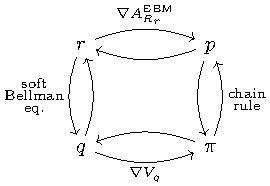
\includegraphics[width=0.7\linewidth]{figures/diagram.pdf} 
 \caption{Summary of mappings discussed in this paper.} 
 \label{fig:diagram} 
 \end{figure}

\section{From the chain rule to Bellman equations}

\subsection{Bijection between distributions} 
 \label{sec:bijection_distributions}

확률의 연쇄 법칙은 결합 확률을 인수분해합니다.
조건부 확률의 곱으로 분배됩니다.
이 섹션에서는 이 방법을 사용하여 절차를 도출하는 방법을 보여줍니다.
임의의 시퀀스 분포 $p \in \cP(\cY|\cX)$를 
다음 토큰 배포 $\pi \in \cP(\augvoc|\cS)$ , 그 반대.

\paragraph{From sequence to next-token distributions.}

$\x \in \cX$ 및 $\y \in \cY$(예: $|\y| = \tau$ )와 $1 \le
\tau \le T$ 의 경우 절차는 연속적으로 주변화 및 조건화를 통해 작동됩니다.
역순으로.  먼저 $p(\y_{\le \tau}|\x) \coloneqq p(\y |
\x)$ 에서 시작하여 $t=\tau-1$ 에서 $t=1$ 까지 정의합니다.
 \begin{equation} 
p( \y _{ \le t}| \x ) \coloneqq \sum _{y_{t+1} \in \augvoc } 
p( \y _{ \le t}, y_{t+1}| \x ).
 \end{equation} 
둘째, 
$t=\tau$에서 $t=2$까지 정의합니다. 
 \begin{equation} 
 \pi (y_t| \x , \y _{<t}) \coloneqq \frac {p( \y _{ \le t}| \x )}{p( \y _{ \le t-1}| \x )},
 \end{equation} 
$\pi(y_1|\x) \coloneqq p(y_1|\x)$로 끝납니다.

\paragraph{From next-token to sequence distributions.}

반대로, 다음 토큰 분포 $\pi \in
\cP(\augvoc|\cS)$ 에서 다음과 같이 시퀀스 분포 $p
\in \cP(\cY|\cX)$ 를 재구성할 수 있습니다.
 \begin{equation} \label{eq:chain_rule_of_proba} 
p( \y | \x ) = \prod _{t=1}^{| \y |} \pi (y_t | \x , \y _{<t}). 
 \end{equation} 
실제로, $\pi$의 정의를 대체함으로써 우리는 다음을 관찰합니다.
제품은 조인트를 정확하게 복구하는 텔레스코픽 시퀀스를 형성합니다.
배포:
 $
\prod_{t=1}^{|\y|} \pi(y_t | \x, \y_{<t}) 
= \frac{p(\y_{\le 1}|\x)}{1} \times
\frac{p(\y_{\le 2}|\x)}{p(\y_{\le 1}|\x)} \times \dots \times \frac{p(\y_{\le
\tau}|\x)}{p(\y_{\le \tau-1}|\x)}
= p(\y|\x)$ .

\paragraph{The chain rule of probability as a bijection.}

$p$ 와 $\pi$ 사이에는 고유한 대응 관계가 있으므로 절차는 다음과 같습니다.
$\cP(\cY|\cX)$ 와 $\cP(\cA|\cS)$ 사이의 전단사를 정의합니다.

\subsection{Bijection in function space} 
 \label{sec:bijection}

이제 EBM 및 ARM에 대한 전단사를 인스턴스화합니다.
시퀀스와 다음 토큰을 사용하는 것으로 볼 수 있음 Gibbs(Boltzmann)
각각 배포. 이 섹션에서는 손실이 없다고 가정합니다.
$R$가 다음과 같이 분해되는 일반성
 \begin{equation} 
 \Rsub{r} ( \x , \y ) \coloneqq \sum _{t=1}^{| \y |} r( \underbrace { \x \oplus \y _{<t}}_{ \s _t}, y_t),
 \label{eq:R_decomposition} 
 \end{equation} 
여기서 $r \colon \cS \times \augvoc \to \RR$는 즉각적인(다음 토큰) 보상입니다.
실제로 $R$가 위와 같이 자연 분해되지 않는다면,
우리는 항상 마지막 단계에서 0이 아닌 모든 보상을 할당할 수 있습니다.

이제 변환하는 방법을 보여드리겠습니다. 
 $r \colon \cS \times \augvoc \to \RR$ 
EBM에서 사용되는
 $q \colon \cS \times \augvoc \to \RR$ 
ARM에서 사용되며 그 반대의 경우도 마찬가지입니다.

\paragraph{From EBM to ARM.}

$r \colon \cS \times \augvoc \to \RR$가 주어졌다고 가정합니다. 
우리는 매핑 $q = \cM(r)$를 다음과 같이 정의합니다.
 \begin{equation} 
q( \s _t, y_t) \coloneqq 
 \begin{cases} 
r( \s _t, y_t) & \mbox{if} ~ y_t = \eos \\
r( \s _t, y_t) + V_q( \s _t \oplus y_t) & \mbox{if} ~ y_t \neq \eos 
 \end{cases},
 \label{eq:q_from_r} 
 \end{equation} 
여기서 $\s_t \in \cS$ 및 $y_t \in \augvoc$ .
그것을 기억해
 \begin{equation} 
V_q( \s _t \oplus y_t) = \underset {y_{t+1} \in \augvoc }{ \lse } ~ q( \s _t \oplus y_t, y_{t+1}). 
 \end{equation} 
$q(\s_t, \cdot)$가 $q(\s_{t+1}, \cdot)$에 의존하여 재귀적 종속성을 생성하는 것을 볼 수 있습니다.
따라서 $r$에서 $q$를 계산하는 작업은 가능한 모든 상태에 대해 $t=\tau$에서 $t=1$까지 순차적으로 수행되어야 합니다.

\paragraph{From ARM to EBM.}

이제 $q \colon \cS \times \augvoc \to \RR$가 주어졌다고 가정합니다. 
역 매핑 $r = \cM^{-1}(q)$를 다음과 같이 정의합니다.
 \begin{equation} 
r( \s _t, y_t) \coloneqq 
 \begin{cases} 
q( \s _t, y_t) & \mbox{if} ~ y_t = \eos \\
q( \s _t, y_t) - V_q( \s _t \oplus y_t) & \mbox{if} ~ y_t \neq \eos 
 \end{cases} .
 \label{eq:r_from_q} 
 \end{equation} 
더 이상 재귀적 종속성이 없으므로
$q$에서 $r$를 계산하는 것은 병렬로 수행될 수 있습니다.

\paragraph{Bijection.}

$\cM$ 매핑과 그 역 $\cM^{-1}$ 매핑을 정의한 후,
이제 결과를 공식적으로 발표할 수 있습니다.

\begin{proposition} [함수 공간에서의 전단사] \label{prop:bijection} 
$q = \cM(r)$ 매핑은 전단사적이며
모든 $\x \in \cX$ 및 $\y \in \cY$에 대해 우리는
 \begin{align} 
    p^ \ebm _{ \Rsub{r} }( \y | \x ) &= p^ \arm _q( \y | \x ) \\
    A^ \ebm _{ \Rsub{r} }( \x ) &= V_q( \x ).
 \end{align} 
 \end{proposition} 
증거는 부록 \ref{proof:bijection}에 나와 있습니다.
이는 EBM이 다음과 같은 형태로 변형될 수 있음을 보여줍니다.
다음 로그 파티션 $V_q$를 추가하여 $r$가 "수정"된 경우 ARM
상태.  MaxEnt RL 용어(섹션 \ref{sec:maxent_rl_perspective} 참조) 
자세한 내용은) $V_q$는 소프트 값 함수로 알려져 있으며 $V_q(\s_t)$는 
$\s_t$ 상태에 있는 미래(소프트) 가치를 캡처합니다. 
따라서 ARM은 EBM을 학습할 수 있는 능력을 갖고 있으므로,
이는 전역적으로 정규화된 분포이고,
ARM은 본질적으로 미래를 내다볼 수 있는 능력을 갖고 있습니다.
$q$를 적절하게 배우십시오.

\paragraph{Computational cost.}

ARM을 EBM으로 변환하는 비용은 $O(VT)$ 입니다.
시퀀스 길이가 선형입니다. 
반면에 EBM을 ARM으로 변환하는 비용은 $O(V^T)$로,
시퀀스 길이. 따라서 EBM을 ARM으로 명시적으로 변환하는 것은 다루기 어렵습니다.
그러나 \ref{sec:minima} 섹션에서 논의할 것처럼 $(\x, \y)$ 쌍에서 학습할 때,
최적의 ARM은 EBM인 \textit{implicitly}이므로 이러한 명시적인 변환은 필요하지 않습니다!

\subsection{Maximum-entropy RL perspective} 
 \label{sec:maxent_rl_perspective}

\paragraph{Autoregressive models as MDPs.}

$\cS$를 상태 집합으로 설정하고 $\cA$를 작업 집합으로 설정합니다.
ARM은 Markov 결정의 특별한 경우로 볼 수 있습니다.
프로세스(MDP)
 \begin{itemize} [topsep=0pt,itemsep=3pt,parsep=3pt,leftmargin=16pt]
 \item 상태는 컨텍스트입니다: $\s_t \coloneqq \x \oplus \y_{<t} \in \cS$ ;
 \item 작업은 토큰입니다: $y_t \in \augvoc$ ;
 \item 다음 상태는 마지막 토큰을 추가합니다.
     $\s_{t+1} \coloneqq \s_t \oplus y_t$ ;
 \item 수평선은 유한하고 붕괴 인자( $\gamma = 1$ )가 없습니다.
 \item $r$는 즉각적인 보상 기능입니다.
 \end{itemize} 
이러한 관점에서 ARM은 특정 인스턴스입니다.
전환 커널 $\mu(\cdot|\s_t, y_t)$가 결정적인 MDP의 경우
$\mu(\s_t \oplus y_t|\s_t, y_t) = 1$로.  이들은 특히
간단한 상태 전환 역학은 각각의
상태는 한 번 이상 방문되지 않습니다. 
이 관점은 (조합적) 맥락적 관점과 혼동되어서는 안 됩니다.
적기 관점(여기서 $\x$는 단일 상태에 해당하고 $\y$는 해당)
행동에 적용하고 $R$는 시퀀스 수준 보상 기능입니다.

\textbf{Soft Bellman equation.} MaxEnt RL에서는 다음 정책을 구합니다.
 \begin{equation} 
 \pi ^ \star = \argmax _{ \pi \in \cP ( \cA | \cS )}    
 \EE \sum _{t=1}^ \infty \gamma ^t (r(S_t, A_t) - \log \pi (A_t | S_t)).
 \label{eq:policy_gradient_objective} 
 \end{equation} 
상태-행동 쌍의 궤적에 대한 기대 
$S_1 \sim p_\cX$부터 시작하여 다음
 \begin{align} 
A_t & \sim \pi ( \cdot | S_t) \\
S_{t+1} & \sim \mu ( \cdot | S_t, A_t).
 \end{align} 
이는 이 문헌에서 잘 알려져 있습니다(자세한 내용은 섹션 \ref{sec:related_work} 참조).
상세 검토) 최적의 솔루션은
 \begin{equation} 
 \pi ^ \star (a| \s ) = \exp (q^ \star ( \s , a) - V_{q^ \star }( \s ))
 \end{equation} 
여기서 $q^\star$는 고정 소수점 방정식의 해입니다.
 \begin{equation} 
q( \s , a) = r( \s , a) + \gamma \EE _{S \sim \mu ( \cdot | \s , a)} V_{q}(S).
 \label{eq:soft_q_learning_objective} 
 \end{equation}

\paragraph{Existence and uniqueness of the fixed point.}

일반적인 RL 설정(무한 지평선, 순환 MDP)에서는 존재와
고정점 $q^\star$의 고유성은 Banach 고정점 정리에 의존합니다.
표준 상태 
이는 단순히 $\gamma < 1$ 입니다. 이는 소프트 Bellman 연산자를 보장합니다.
 $(\mathcal{B}_r q)(\s, a) \coloneqq r(\s, a) + \gamma \EE_{S \sim \mu(\cdot |
\s, a)} V_{q}(S)$는 수축 매핑입니다.
일반적으로 $q^\star$는 명시적인 공식을 사용하지 않으며
$q^\star$를 찾으려면 어떤 형태의 고정 소수점 반복이 필요합니다.
대조적으로, 우리의 설정(유한 지평선, 비순환 MDP)에서는 
 $q^\star = \cM(r)$는 고정 소수점 해의 명시적 공식입니다.
존재성과 고유성(가역성)을 모두 보장합니다.
또한, 확률의 연쇄 법칙을 통해 전단사를 구성했는데,
소프트 벨만 방정식으로 깊은 연관성을 밝히다
우리의 특별한 환경에서.

\subsection{Entropy-regularized DP on a DAG perspective} 
 \label{sec:dp_dag}

우리는 또한 우리의 전단사를 정규화된 동적 프로그래밍(DP)으로 볼 수도 있습니다.
방향성 비순환 그래프(DAG).  이러한 관점에서 우리는 DAG를 정의합니다.
 \begin{itemize} [topsep=0pt,itemsep=3pt,parsep=3pt,leftmargin=16pt]
 \item $\s_1 = \x$ 에 해당하는 하나의 시작(루트) 노드가 있습니다.
 \item에는 하나의 끝 노드가 있습니다.
 \item 중간 노드는 컨텍스트 $\s_t \coloneqq \x \oplus \y_{<t}$ 입니다.
 \item 간선 가중치는 $y_t$를 추가한 $r(\s_t, y_t)$ 값을 나타냅니다.
    context $\s_t$ (높을수록 좋음);
 \item 노드 $\s_t \coloneqq \x \oplus (y_1, \dots, \eos)$는
    끝 노드에 연결된 가중치 $0$의 단일 나가는 edge를 갖는다.
 \end{itemize}  
컴퓨팅
 $\max_{\y \in \cY} \sum_{t=1}^{|\y|} r(\x \oplus \y_{<t}, y_t)$  
그런 다음 DAG에서 최대값의 경로를 찾는 것과 같습니다.
로그 파티션을 계산합니다.
 $A^\ebm_{\Rsub{r}}(\x) 
= \underset{\y \in \cY}{\lse} ~ \sum_{t=1}^{|\y|} r(\x \oplus \y_{<t}, y_t)$ 
{ \em 소프트} 최대값의 경로를 찾는 것과 같습니다.

\paragraph{Top-down vs.\ bottom-up DP.}

소프트 최대값을 계산하려면 
 $A^\ebm_{\Rsub{r}}(\x) = V_q(\x)$ 
DP의 $q = \cM(r)$의 경우 두 가지 접근 방식이 가능합니다.
\textit{top-down} DP에서는 원하는 수량인 $V_q(\x)$부터 시작합니다.
계산하고 재귀합니다. 이는 DAG를 시간상 앞으로 이동하는 것에 해당합니다.
\textit{bottom-up} DP(표)에서는 기본 사례에서 시작하여
$V_q(\x)$까지 .  이는 DAG를 시간상 뒤로 이동하는 것에 해당합니다.
\citep{mensch2018differentiable} 에 표시된 것처럼
log-sum-exp와 log-sum-exp에 대한 $+$의 분포는 다음을 보장합니다.
동적 프로그래밍의 최적성. 실제로 우리는 ($|\y| = T$를
표기를 단순화한다)
 \begin{small} 
 \begin{align} 
A^ \ebm _{ \Rsub{r} }( \x )
&= \underset{\y \in \cY} { \lse } ~ \sum _{t=1}^T r( \x \oplus \y _{<t}, y_t) \\
&= \underset{y_1 \in \cV} { \lse } \dots \underset{y_T \in \cV} { \lse } ~
 \sum _{t=1}^T r( \x \oplus \y _{<t}, y_t) \\
&= \underset{y_1 \in \cV} { \lse } ~ \biggl [ r( \x , y_1)
+ \dots + \underset{y_T \in \cV} { \lse } ~ \Bigl [ r( \x \oplus \y _{<T}, y_T) \Bigr ] \biggr ].
 \end{align} 
 \end{small} 
로그 분할의 기울기가 정확히 일치한다는 것은 잘 알려져 있습니다.
한계 확률 \citep{wainwright2008graphical} .
부록 \ref{sec:backpropagation}에서,
우리는 그라디언트 \wrt $r$를 보여줍니다.
 $q = \cM(r)$의 $A^\ebm_{\Rsub{r}}(\x) = V_q(\x)$는 실제로 정확히 일치합니다.
응답 접두어의 한계 확률.

\section{Theoretical analysis}

\subsection{Learning EBMs and ARMs from input-output pairs} 
 \label{sec:minima}

이 섹션에서는 
섹션 \ref{sec:bijection}의 전단면을 토대로 구축,
우리는 EBM 학습과 ARM 학습 사이의 동등성 결과를 기술합니다.
 $(\x, \y)$ 쌍.

\paragraph{Negative log-likelihood of EBMs.}

$p^\ebm_R$에 따라 $\x$가 주어졌을 때 $\y$의 음의 로그 우도는 다음과 같습니다.
 \begin{equation} \label{eq:lebm} 
 \ell ^ \ebm _R( \x , \y ) 
 \coloneqq - \log p^ \ebm _R( \y | \x ) 
= A^ \ebm _R( \x ) - R( \x , \y ).
 \end{equation} 
손실은 $R$에서 볼록하며 속성을 만족합니다.
 \begin{equation} 
 \ell ^ \ebm _R( \x , \y ) = 0 \iff p^ \ebm _R( \y | \x ) = 1.
 \end{equation}

\paragraph{Negative log-likelihood of ARMs.}

다음에 따라 $\x$가 주어졌을 때 $\y$의 음의 로그 우도는 다음과 같습니다.
 $p^\arm_q$는
 \begin{align} 
 \ell ^ \arm _q( \x , \y )
& \coloneqq - \log p^ \arm _q( \y | \x ) \\
&= A^ \arm ( \x , \y ) - \Qsub{q} ( \x , \y ).
 \end{align} 
손실은 $q$에서 볼록하며 속성을 만족합니다.
 \begin{equation} 
 \ell ^ \arm _q( \x , \y ) = 0 \iff p^ \arm _q( \y | \x ) = 1.
 \end{equation}

$A^\ebm$ 와 달리 $A^\arm$ 는 $\x$ 뿐만 아니라 $\x$ 및 $\y$ 의 함수입니다.
따라서 EBM과 달리 ARM의 음의 로그 우도는 다음을 사용합니다.
지상 진실 시퀀스 $\y$를 경로로 사용합니다. 이것은 \textbf{teacher
forcing}로 알려져 있습니다. 이름에서 알 수 있듯이 이러한 행동은 다음과 같이 자연스럽게 발생합니다.
ARM에서 음의 로그 우도를 사용한 결과.

\paragraph{Equivalence of minima.}

예상되는 위험을 정의합시다
 \begin{align} 
 \cL ^ \arm (q) & \coloneqq \EE _{(X,Y) \sim \rho } \left [ \ell ^ \arm _q(X, Y) \right ] 
 \label{eq:expected_risk_arm} \\
 \cL ^ \ebm (R) & \coloneqq \EE _{(X,Y) \sim \rho } \left [ \ell ^ \ebm _R(X, Y) \right ]. 
 \label{eq:expected_risk_ebm} 
 \end{align} 
그러면 우리는 다음과 같은 동등성을 갖게 되는데, 이는 간단한 결과입니다.
섹션 \ref{sec:bijection}에서 우리의 전단사를 설명합니다.
 \begin{proposition} [최소값의 등가] \label{prop:same_minima}

$\cX \times \cY$에 대한 공동 분포 $\rho$에 대해 다음을 얻습니다.
 \begin{align} 
 \min _{q \in \cF ( \cS \times \augvoc )} \cL ^ \arm (q)
&= 
 \min _{r \in \cF ( \cS \times \augvoc )} 
 \cL ^ \ebm ( \Rsub{r} ) \\
&= 
 \min _{R \in \cF ( \cX \times \cY )} 
 \cL ↑ \ebm (R)
 \end{align} 
그리고 $q^\star = \cM(r^\star)$를 사용하면
 \begin{small} 
 \begin{align} 
q^ \star \in \argmin _{q \in \cF ( \cS \times \augvoc )}
 \cL ^ \arm (q) 
& \iff 
r^ \star \in \argmin _{r \in \cF ( \cS \times \augvoc )} 
 \cL ^ \ebm ( \Rsub{r} ) \\
& \implies 
 \Rsub{r^\star} \in \argmin _{R \in \cF ( \cX \times \cY )} 
 \cL ^ \ebm (R).
 \end{align} 
 \end{small} 
 \end{proposition} 
증거는 부록 \ref{proof:same_minima}를 참조하세요.
제안 \ref{prop:same_minima}는 목표가 모델을 적합하는 것일 때 다음을 보여줍니다.
음의 로그 우도 최소화를 통해 관찰된 입력-출력 쌍 $(\x, \y)$, EBM 및
ARM은 최소화를 수행한다면 동등하게 강력합니다.
함수 공간(function space)은 함수가 데이터에 적합할 수 있음을 의미합니다.
완벽하게.

\paragraph{Optimality of teacher forcing.}

데이터에서 보상 $R$를 학습하는 것은 \textbf{inverse RL} 설정에 해당합니다.
 \citep{ziebart2008maximum} .  이중성 관점에서 \citep{sander2025joint},
최적의 원변수 $R^\star$는 최적의 이중 변수에 연결됩니다.
 $p^\star$부터 모든 $\x \in \cX$에 대해,
 \begin{equation} 
p^ \star ( \cdot | \x ) 
= \mathrm{softargmax} (R^ \star ( \x , \cdot )) 
= p^ \ebm _{R^ \star }( \cdot | \x ). 
 \end{equation} 
안타깝게도 $R^\star$에서 $p^\star$를 복구하는 것은 어렵습니다.
다루기 힘든 정규화 상수.  그러나 $q^\star$가 주어지면(최적
교사 강제를 통한 솔루션), $p^\star$는 $\pi_{q^\star}$에서 구성될 수 있습니다. 
\eqref{eq:chain_rule_of_proba} 에서 확률의 연쇄 규칙을 사용하여,
 \begin{equation} \label{eq:p_star_from_q_star} 
p^ \star ( \y | \x ) = \prod _{t=1}^{| \y |} \pi _{q^ \star }(y_t | \x , \y _{<t}). 
 \end{equation} 
이는 기능을 최적화할 때 교사 강제가 최적이라는 것을 보여줍니다.
공간. $\cM$ 매핑은 완전히 암시적이라는 점을 강조합니다.
이 경우에는 (명시적으로 계산할 필요가 없습니다).
그림 \ref{fig:diagram}에 매핑을 요약합니다.

\subsection{Distilling EBMs into ARMs}

우리는 \ref{sec:unified_perspective} 섹션에서 KL 정규화 RL이 가능하다는 것을 보았습니다.
EBM을 ARM으로 증류하는 것으로 간주됩니다.  이는 근사치의 필요성을 유발합니다.
ARM의 EBM 보장.

\paragraph{Function space.}

다르게 말하면, 제안 \ref{prop:bijection}는 정확한 내용을 보여줍니다.
$q = \cM(r)$ 매핑은 다음을 만족합니다.
모든 $\x \in \cX$에 대해  
 \begin{equation} 
 \KL (p^ \arm _q( \cdot | \x ), p^ \ebm _{ \Rsub{r} }( \cdot | \x )) = 0.
 \end{equation} 
이러한 결과는 함수 공간에서도 유지됩니다.  이것은 소위 표 형식 설정입니다.
$q \colon \cS \times \augvoc \to \RR$ 및 $r \colon \cS
\times \augvoc \to \RR$ 함수가 (거대한) 배열로 표현되는 RL.
컨텍스트(상태) $\cS$의 공간과 다음 토큰의 공간이 있다는 사실
 $\augvoc$는 유한합니다.

\paragraph{Function approximation setting.}

실제로 $q$ 및 $r$는 매개변수화된 함수를 사용하여 구현됩니다.  이에
설정에 따라 더 이상 EBM과 ARM 간의 정확한 변환이 불가능할 수 있지만
KL 발산을 묶을 수 있습니다.
 \begin{proposition} [KL행]
모두를 위해
 $r \colon \cS \times \augvoc \to \RR$,
 $q \colon \cS \times \augvoc \to \RR$ 
그리고
 $\x \in \cX$, 우리는
 \begin{equation} 
 \KL (p^ \arm _q( \cdot | \x ), p^ \ebm _{ \Rsub{r} }( \cdot | \x ))
 \le 2T \max _{ \substack{\s \in \cS(\x)\\y \in \augvoc} } |q^ \star ( \s , y) - q( \s , y)|,
 \end{equation} 
어디서
 $q^\star \coloneqq \cM(r)$ .
 \label{prop:kl_bound} 
 \end{proposition} 
증거는 부록 \ref{proof:kl_bound}에 나와 있습니다.
KL 발산은 대칭이 아니라 동일한 경계입니다. 
에도 적용됩니다
 $\KL(p^\ebm_{\Rsub{r}}(\cdot|\x), p^\arm_q(\cdot|\x))$ .

\paragraph{Approximation using a Transformer.}

$\Rsub{r}$ 로 매개변수화된 고정 EBM의 경우 $q^\star = \cM(r)$ 로 설정합니다.  우리는 이제 그것을 보여줍니다
 $q^\star$는 다음을 활용하여 인과 변환기 모델로 근사화할 수 있습니다.
인과 변환기에 의한 인과 매핑의 강력한 근사 결과
 \citep[Theorem 2]{furuya2024transformers} .  보다 정확하게는 모든 $\varepsilon
> 0$에 대해 다음과 같은 인과 변환기 $\mathcal{T}: \cS \to \RR^{|\augvoc|}$가 존재합니다.
모든 $\x \in \cX$에 대해 
 \begin{equation} 
 \max _{ \substack{\s \in \cS(\x), y \in \augvoc} }|q^ \star ( \s ,y)- \mathcal{T} ( \s )[y]| \leq \varepsilon .
 \end{equation} 
제안 \ref{prop:kl_bound}와 함께 이는 모든 $\x \in \cX$에 대해 다음을 제공합니다.
 \begin{equation} 
 \KL (p^ \arm _{ \mathcal{T} (.)[.]}( \cdot | \x ), p^ \ebm _{ \Rsub{r} }( \cdot | \x ))
 \le 2T \varepsilon .
 \end{equation} 
그러나 이 결과에는 $\cT$의 임베딩 차원이 필요합니다.
어휘 크기 $|\mathcal{V}|$ \citep{furuya2024transformers} 로 확장합니다.

\section{Numerical validation}

이 섹션에서는 합성 소형 언어 모델을 사용하여 이론을 검증합니다. 우리
작은 어휘 $V$ 및 작은 최대 길이 $T$에 중점을 두고 정확한
근사치에 의존하지 않고 EBM의 로그 파티션 계산
알고리즘.  \eqref{eq:expected_risk_arm}에서 예상되는 위험을 최소화하고
 \eqref{eq:expected_risk_ebm} , EBM에 대해 비인과적 변환기를 사용하고
ARM을 위한 인과 변환기. 
최소 위험은 $\cL^\star \coloneqq -\EE_{(X,Y) \sim \rho} \log
\rho(X, Y)$ 로 정의됩니다. 모든 실험 세부 사항은
부록~ \ref{app:exp_details} .

\begin{figure} [t]
     \centering 
     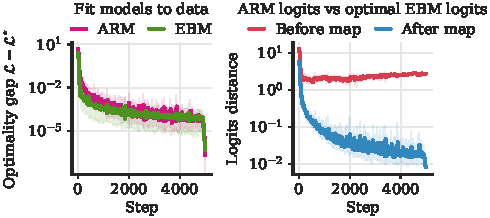
\includegraphics[width=\linewidth]{figures/cvg_and_logits_dist_V8_T4_N3_main.pdf} 
     \caption {명제 \ref{prop:same_minima}의 실증적 검증 .
     \textbf{Left} : ARM 및 EBM의 예상 위험 최소화
인과 및 비인과 변환기에 의해 각각 매개변수화됩니다.
 \textbf{Right} : 훈련된 ARM의 로지트와 $L_\infty$ 사이의 거리
매핑 적용 전후의 \textbf{optimal} EBM의 로지트
 $\cM$ .}
     \label{fig:ebm_arm_bij_illus} 
 \end{figure}

그림 ~ \ref{fig:ebm_arm_bij_illus}(왼쪽)에서는 EBM과 ARM 모두의 최적성 격차 $\cL -
\cL^\star$를 최적화 단계의 함수로 표시합니다.  우리의
결과는 EBM과 ARM이 예측한 대로 동일한 최소값에 수렴함을 확인합니다.
제안으로~ \ref{prop:same_minima} .  아마도 더 놀랍게도 우리의 결과는
또한 전체 기간 동안 두 모델의 손실 곡선이 매우 가깝다는 것을 보여줍니다.
훈련 과정.  이러한 결과는 여러 모델 크기에서 확인되었으며
시퀀스 길이/어휘 비율(부록~ \ref{app:exp_details}).

그림~ \ref{fig:ebm_arm_bij_illus}(오른쪽)에서는 $L_\infty$ 거리를 보여줍니다.
훈련된 ARM의 로지트와 최적 EBM의 로지트 사이
그리고 $\cM$ 매핑을 적용한 후.  따라서 우리의 결과는
$\cM$ 매핑을 사용하여 EBM 및 ARM의 로짓을 명시적으로 변환할 수 있습니다.
그러나 우리는 명시적인 로짓 변환이 필요하지 않다는 점을 강조합니다.
또한 \eqref{eq:p_star_from_q_star}를 사용하여 EBM 분포를 인수분해합니다.

\section{Related work} 
 \label{sec:related_work}

\paragraph{Maximum-entropy RL.}

최대 엔트로피는 역 RL에 사용되었으며 목표는 보상을 복구하는 것입니다.
오프라인 궤적 \citep{ziebart2008maximum}의 기능.  앞으로
설정의 선구자는 동적 정책 프로그래밍 \citep{azar2012dynamic} 입니다.
이후 많은 논문에서 두 가지 사이의 동등성을 공식적으로 확립했습니다.
\eqref{eq:policy_gradient_objective}를 해결하려는 정책 기반 방법 
 \wrt $\pi$ 및 가치 기반 방법으로 만족을 추구합니다.
 \eqref{eq:soft_q_learning_objective} \wrt $q$ 
 \citep{o2016pgq,haarnoja2017reinforcement,nachum2017bridging,schulman2017equivalence} .
볼록 이중성을 사용하여 연속 동작 공간에서 등가성을 재검토했습니다.
 \citep{richemond2017short} .
엔트로피 정규화 RL은 \citep{neu2017unified}에 대해 추가로 연구되었으며 확장되었습니다.
다른 강하게 볼록한 정규화 장치 \citep{geist2019theory} .
여러 논문에서는 1단계 및 다단계 일관성 손실 함수 기반을 제안했습니다.
최적 조건에 손실 제곱을 적용하면
 \eqref{eq:soft_q_learning_objective} 
 \citep{nachum2017bridging,schulman2017equivalence,clavier2025shiq} .
여러 논문에서 소프트 액터 비평 알고리즘을 제안했습니다.
 \citep{o2016pgq,haarnoja2017reinforcement,haarnoja2018soft} 또는 공동 학습
정책 및 가치 함수 \citep{richemond2024offline} .


\paragraph{RL as probabilistic inference.}

Maxent RL은 다음을 사용하여 확률적 추론 관점에서 볼 수 있습니다.
방향이 지정되지 않은 그래픽 모델
 \citep{toussaint2009probabilistic,ziebart2010modeling} , EBM 정의( \aka 
조건부 무작위 필드) 또는 방향성 그래픽 모델, 미러링 숨김
마르코프 모델 \citep{attias2003planning,levine2018reinforcement} .  특히,
이 연결은 MCTS를 사용하여 추론 문제를 해결하는 데 활용되었으며
학습된 소프트 값 함수 \citep{buesing2020approximate} .  반대로,
maxent RL을 위해 확률적 추론 도구를 활용할 수 있습니다.
 트위스트 순차 몬테카를로와 같은 \citep{korbak2022rl}
 \citep{zhao2024probabilistic} .
우리는 우리의 환경에서 확률적 추론 관점을 다시 살펴봅니다.
부록 \ref{sec:proba_inference_perspective}에서.

\paragraph{Energy-based models.}

확률론적으로 $(\x, \y)$ 쌍에서 EBM을 학습하기 위한 표준 접근 방식
경사하강법에는 EBM \citep{song2021train} 에서 샘플링이 필요합니다.
일반적으로 $\cY$가 연속적일 때 Langevin과 같은 MCMC 알고리즘이 포함됩니다.
$\cY$가 이산적일 때 Gibbs 샘플링. 이 접근 방식은 함수 $R$(역 RL의 보상, 섹션 \ref{sec:minima} 참조)를 학습하므로
EBM에서 샘플을 생성하려면 생성 모델 $\pi$, MCMC가 필요합니다.
학습된 $R$에 의해 매개변수화됩니다.  min-min 공식이 공동으로 제안되었습니다.
$R$ 및 로그 파티션 $A$ \citep{sander2025joint} 를 배우십시오. 이것이 우회하는 동안
열차 시간에 MCMC가 필요하지만 EBM에서 샘플링하려면 여전히 MCMC가 필요합니다.
그러나 우리는 샘플링이 필요하지 않고 단지 예측만 할 필요가 있다면 강조합니다.
EBM의 모드($\x$가 주어지면 $\y$가 가장 가능성이 높은 출력)인 경우에만 필요합니다.
로그 파티션을 포함하지 않고 일부에서는 다루기 쉬운 $R$를 최대화합니다.
$\cY$를 설정합니다.  반면에 최소-최대 공식은 공동으로 사용될 수 있습니다.
$(\x,
\y)$ 쌍 \citep{ho2016generative} 에서 판별자(보상) $R$ 및 생성자(정책) $\pi$를 학습합니다. 이러한 접근 방식에는 다음과 같은 경우 MCMC가 필요하지 않습니다.
생성기는 ARM의 경우처럼 설계에 따라 쉽게 샘플을 생성합니다.

\paragraph{GFlowNets.}

GFloNets \citep{bengio2021flow,bengio2023gflownet}를 사용하여 다음을 수행할 수 있습니다.
상각된 확률적 추론 \citep{hu2023amortizing} . 흐름 일관성 방정식은 동일한 역할을 합니다.
Soft Bellman 방정식으로 일관성 손실 함수 설계 가능
 \citep{malkin2022trajectory} .  실제로 최근 연구에 따르면
일반 DAG 설정에서도 GFlowNets를 MaxEnt RL로 캐스팅할 수 있습니다.
 \citep{tiapkin2024generative} .

\paragraph{Limitations of teacher forcing.}

최근 연구에서는 다음 토큰 예측 목표(교사 강제)가 다음과 같다고 주장했습니다.
구조적으로 "근시안적"이며 미래 가치 정보를 역전파하지 못합니다.
효과적으로 \citep{bachmann2024pitfalls} 계획에 실패하게 됩니다.  에서
대조적으로, 명제 \ref{prop:same_minima}는 다음의 전역 최소값을 보여줍니다.
교사는 목표(기능 공간에서) \textit{is} EBM을 강제합니다.
본질적으로 파티션 함수 $V_q$를 통해 미리보기를 수행합니다. 우리의 일
그러므로 교사 강요의 한계는 교사의 강요에 국한되지 않는다는 것을 암시한다.
목표 그 자체이지만 최소값에 도달하기가 어렵기 때문에
최적화 또는 근사 오류.  이는 다음을 보여주는 이전 작업과 일치합니다.
계획 실패는 약한 상관 관계에 대한 과적합에서 비롯됩니다.
본질적인 구조적 무능력보다는 감독
 \citep{frydenlund2024mystery} .
보완 작업에서 RL의 교사 강제에 대응하는 행동 복제가 지평선 독립적인 샘플 복잡성을 달성하는 것으로 나타났습니다.
 \citep{foster2024behavior} .

\section{Conclusion}

\paragraph{Significance of this work.}

EBM과 ARM은 일반적으로 두 가지 매우 다른 클래스의 모델로 간주됩니다.  EBM
전역적으로 일관성이 있지만 훈련 및 샘플링이 어렵습니다. 반면 ARM은
훈련하고 샘플링하기는 쉽지만 과거를 되돌아볼 뿐입니다.  우리의 논문
EBM과 ARM이 실제로 밀접하게 관련되어 있음을 보여줍니다.  우리의 첫 번째 기여
기능적으로 EBM과 ARM 사이의 전단사 매핑 $\cM$를 설정하는 것입니다.
공간.  이 매핑은 일반적으로 소프트 벨만 방정식의 특별한 경우이지만
MDP(섹션 \ref{sec:maxent_rl_perspective} ) 및 엔트로피 정규화
DAG(섹션 \ref{sec:dp_dag})의 동적 프로그래밍을 통해 우리는
확률의 연쇄 법칙과 매우 다른 각도(섹션
 \ref{sec:bijection_distributions} 및 섹션 \ref{sec:bijection}).  언제
$(\x, \y)$ 쌍으로부터 학습하면, 명제 \ref{prop:same_minima}는 다음을 보여줍니다.
기능 공간에서 EBM과 ARM은 동등하게 강력합니다.
이 경우 교사 강제의 최적성.  EBM 교사를 증류할 때
ARM 학생, 
제안
 \ref{prop:kl_bound}는 EBM과 ARM 사이의 KL이 다음과 같이 제한됨을 보여줍니다.
전단사 매핑 $\cM$ 의 $L_\infty$ 표준.
수치 실험을 통해 검증된 우리의 결과는
다음 토큰 예측에 대한 정당성을 제공합니다.
패러다임과 교사 강요.

\paragraph{Limitations.}

$(\x, \y)$ 쌍에서 학습할 때 제안 \ref{prop:same_minima} 
$R$를 최적화할 때 ARM과 EBM이 동등하게 강력하다는 사실을 입증했습니다.
 함수 공간의 $q$. 그러나 실제로 $R$는
$q$는 인과관계가 아닌 변압기여야 합니다.  또한, 제안
 \ref{prop:bijection}는 ARM과 EBM이
이에 상응하는 $q$ 는 $q(\s, y) = r(\s, y) + V_q(\s \oplus y)$ 형식을 취해야 합니다.
여기서 $V_q$는 모든 향후 연속의 (소프트) 최적 값을 나타냅니다. 는
따라서 함수 $q$는 이중 작업을 수행해야 합니다.
로컬 점수 $r$ 이며 잠재적으로 복잡한 것을 암시적으로 계산하는 방법을 배워야 합니다.
미래지향적 가치함수 $V_q$(가능한 모든 미래를 무시함)
역방향 아키텍처만을 사용합니다.  
제안 \ref{prop:same_minima}는 최적화 또는
근사 오류.
복잡성을 공식적으로 비교
$R$를 학습하는 것과 $q$를 학습하는 것이 유망한 미래 방향입니다.
또 다른 중요한 방향은 잠재 변수의 영향을 연구하는 것입니다(사고
흔적) ARM의 표현력을 향상시킵니다.

\paragraph{Bridging communities.}

이 문서에서는 ARM, EBM 및 Maxent RL 간의 브리지를 구축합니다.
우리의 논문이 얼마나 많은
작품과 관점은 서로 연관되어 있다.

\section*{Impact statement}

이 논문은 에너지 기반 모델과 자기회귀 모델 간의 연결을 연구하여 다음 토큰 예측의 예측 기능을 정당화합니다. 
우리는 이 작업에서 직접적으로 발생하는 특정 윤리적 또는 사회적 영향을 예상하지 않습니다.

\bibliography{main}
\bibliographystyle{icml2026}


\newpage
\appendix
\onecolumn

\section{Supplementary materials} 
 \label{sec:supp_material}

목차:
 \begin{itemize} [topsep=0pt,itemsep=3pt,parsep=3pt,leftmargin=16pt]

\item 가변 길이 시퀀스 처리 
 \begin{itemize} 
     \item ARM (섹션 \ref{sec:variable_length_handling}).
     \item EBM (섹션 \ref{sec:variable_length_handling_ebms}).
 \end{itemize} 
 \item 체인 규칙 
 \begin{itemize} 
     \item 엔트로피의 연쇄 법칙(\ref{sec:chain_rule_of_entropy} 섹션).
     \item KL의 체인 규칙(섹션 \ref{sec:chain_rule_of_kl}).
 \end{itemize} 
 \item 전단사
 \begin{itemize} 
 \item 참조 측정을 사용한 전단사 
    (섹션 \ref{sec:bijection_with_ref_measure}).
 \item 확률 관점의 연쇄 법칙 
    (섹션 \ref{sec:bijection_chain_rule_perspective}).
 \item 변형 관점 
    (섹션 \ref{sec:bijection_variational_perspective}).
 \item 적대적 및 변형적 추론 관점 
    (섹션 \ref{sec:bijection_adversarial_perspective}).
 \item 확률적 추론 관점 
    (섹션 \ref{sec:proba_inference_perspective}).
 \end{itemize} 
 \item 그라디언트 
 \begin{itemize} 
     \item 그라디언트 맵(섹션 \ref{sec:gradient_maps} ).
     \item 역전파(\ref{sec:backpropagation} 섹션).
 \end{itemize}

\end{itemize}

\subsection{Handling variable-length sequences in ARMs} 
 \label{sec:variable_length_handling}

완전성을 위해 여기에서 유효한 유도를 유도하는 \eos의 중요한 역할을 검토합니다.
유한한 크기의 가변 길이 시퀀스에 대한 확률 분포.  자세한 내용은
독자에게 \citet[Section 2.5]{cotterell2023formal}를 참조하십시오.  또한보십시오
 \citet[Chapter 6]{eisenstein2019introduction}에 대한 간단한 소개
언어 모델.

\paragraph{Probability of finished vs.\ unfinished responses.}

어휘 $\cV$에서 최대 $T$ 크기까지 가능한 시퀀스 집합을 정의해 보겠습니다. 
$\cV^{\le T} \coloneqq \cup_{t=1}^T \cV^t$로. 
프롬프트의 무작위 변수를 나타내기 위해 $X \in \cX$를 사용하고 다음 크기의 \textbf{finished} 응답의 무작위 변수를 나타내기 위해 $Y \in \cV^{\le
T}$를 사용합니다.
대부분의 $T$.  그런 다음 시퀀스 $\y=(y_1, \ldots,
y_\tau)$가 $\x$에 대해 완료된 응답일 확률을 다음과 같이 정의합니다.
\[
 \PP (Y= \y |X= \x ) \coloneqq \PP (Y_1=y_1, \ldots , Y_ \tau =y_ \tau , \len (Y)= \tau |X= \x).
\]
문장의 길이가 $0 \le \tau \le T$ 인 $Y$ 의 첫 번째 $\tau$ 토큰이 $y_1, \ldots,
y_\tau$ \textbf{and} 일 확률입니다.

이 확률을 \textbf{marginal probability}와 혼동해서는 안 됩니다. 
\textbf{unfinished response}의,
\[
 \PP (Y_{ \le \tau }= \y |X= \x ) \coloneqq \PP (Y_1=y_1, \ldots , Y_ \tau =y_ \tau |X= \x).
\]
$Y$ 의 첫 번째 $\tau$ 토큰이 $y_1, \ldots,
y_\tau$ 인 반면 $Y$ 는 잠재적으로 더 긴 길이일 확률입니다.  공식적으로 이번 행사는 
 $\{Y_1=y_1, \ldots, Y_\tau=y_\tau, \len(Y)=\tau'\}$  
에 대한 
 $\tau' > \tau$ 
싱글톤은 아니지만 이벤트는 
 $\{Y_1=y_1, \ldots, Y_\tau=y_\tau, \len(Y)=\tau\}$  
싱글톤 $\{Y=\y\}$ 로 줄어듭니다. 
다르게 말하면, 
 $\{Y_{\le \tau} = \y\} \neq \{Y=\y\}$ .

\paragraph{Explicit length handling.}

가변 길이의 완성된 응답을 설명하는 자연스러운 방법은 다음과 같습니다.
길이를 인코딩하는 무작위 변수 $L \in \NN$를 정의하고
$l \in \NN$에 대한 고정 크기 시퀀스 $Y_{1:l}|L=l$에 대한 분포입니다.
불행하게도 자동 회귀 설정에서는 정보 흐름이 중단됩니다.
토큰 출력을 시작하기 전에 최종 길이를 예측하지 않습니다. 대신,
자기회귀 모델은 과거 토큰의 길이를 조절할 수 있습니다.
확률 $\PP(Y=\y |X=\x)$를 다음과 같이 분해할 수 있습니다.
 \begin{align*} 
 \PP (Y= \y |X= \x ) & = \PP (Y_1 = y_1, \ldots , Y_ \tau =y_ \tau | X= \x )
 \PP ( \len (Y)= \tau | X= \x , Y_1 = y_1, \ldots , Y_ \tau =y_ \tau ) \\
& = \PP (Y_1 = y_1 |S_1 = \s _1) \ldots \PP (Y_ \tau =y_ \tau | S_ \tau = \s _ \tau )
 \PP ( \len (Y)= \tau | S_ \tau = \s _ \tau ),
 \end{align*} 
컨텍스트(상태)를 사용한 곳
 $\s_t \coloneqq \x \oplus \y_{<t}$ 및 $\s_1 = \x$,
$S_t$ 및 $S_1$의 경우에도 유사합니다.

\paragraph{Implicit length handling using EOS.}

이 분해는 길이를 인코딩하는 간단한 방법을 제안합니다.
자동회귀 모델: \eos라는 새로운 가능한 출력 토큰을 추가합니다.
모든 $t\geq 0$에 대해, 
 \begin{equation} 
 \PP (Y_t = \eos | S_t = \s _t) = \PP ( \len (Y) = t |S_t = \s _t).
 \end{equation} 
이 접근 방식을 사용하면 완성된 응답에는 항상 \eos가 포함되어야 합니다.
마지막 토큰이며 이제 시퀀스 길이에 \eos 가 포함됩니다.  좀 더 공식적으로,
$Y \in \cV^{\le T}$ 를 정의하는 대신 이제 $Y \in \cY$ 를 정의합니다. 여기서 $\cY =
\cup_{t=1}^T (\cV^t \times \{\eos\})$ 입니다.  $\eos$는 단지
길이를 인코딩하는 편리한 방법이며 카디널리티를 변경하지 않습니다.
가능한 시퀀스 세트, 이후
 \begin{equation} 
| \cV ^t \times \{ \eos \}| =| \cV ^t| = V^t.
 \end{equation} 
\eos 접근 방식의 장점은 두 가지 모두를 원활하게 지원할 수 있다는 것입니다.
완료된 응답의 확률(마지막 토큰으로 \eos를 추가하여) 및
미완성 응답의 한계 확률(\textbf{not}에 \eos를 다음과 같이 추가)
마지막 토큰). 실제로 $y_\tau \neq \eos$ 를 가정하면
 \begin{equation} 
 \PP (Y_{ \le \tau }= \y |X= \x ) 
= \PP (Y_1 = y_1 |S_1 = \s _1) \ldots \PP (Y_ \tau =y_ \tau | S_ \tau = \s _ \tau ).
 \end{equation}


$\pi_q$를 정의하는 데 사용되는 $q$ 함수는 (컨텍스트, 다음 토큰) 쌍을 취하고
스칼라 값 점수를 반환합니다.
엄밀히 말하면 컨텍스트 토큰은 $\cV$ 어휘에 있고 다음 토큰은
토큰은 증강 어휘 $\cA \coloneqq \cV \cup \{\eos\}$ 에 있습니다.
따라서 $q \colon \cS \times \cA \to \RR$ 이며, 여기서 $\cS \coloneqq \cup_{t=1}^T
\cX \times \cV^t$ 입니다.

\paragraph{Validity of the probability distribution over sequences.}

우리는 공식적으로 ARM을 보장하는 충분 조건을 제공합니다.
완료된 응답에 대한 유효한 확률 분포를 정의합니다.
 \begin{proposition} [ARM이 정의한 분포의 유효성] \label{prop:valid_arm_proba}

$\cY \coloneqq \bigcup_{\tau=1}^T \voc^{\tau-1} \times \{\eos\}$를 세트로 설정
최대 $T$ 길이의 유효한 완료된 응답 수입니다.  만약 $\pi_q(\eos|\s_T) = 1$라면 
모든 $\s_T \in \cX \times \voc^{T-1}$에 대해, 모든 $\x \in \cX$에 대해 
 \begin{equation} 
 \sum _{ \y \in \cY } p^ \arm _q( \y | \x ) = 1.
 \end{equation} 
즉, ARM은 완료됨에 대한 유효한 확률 분포를 정의합니다.
최대 $T$ 길이의 응답.
 \end{proposition} 
증거는 부록 \ref{proof:valid_arm_proba}에 나와 있습니다.

$\pi_q(\eos|\s_T) = 1$ 조건을 시행하기 위해 다음과 같이 $q$를 정의할 수 있습니다.
 \eqref{eq:q_last_token} .





\subsection{Handling variable-length sequences in EBMs} 
 \label{sec:variable_length_handling_ebms}

\paragraph{Probability of finished vs.\ unfinished responses.}

완료된 응답에 대한 확률을 정의하는 것은 다음과 같이 더 간단합니다.
EBM은 가능한 모든 $\y \in
\cY$에 대해 $\PP(Y=\y |X=\x)$를 직접 매개변수화할 수 있습니다.  EBM의 음에너지 $R$는 일정한 인자까지
$X=\x$ 가 주어지면 싱글톤 이벤트 $\{Y=\y\}$ 의 로그 확률, 
 \begin{equation} 
R( \x , \y ) = \log \PP (Y= \y |X= \x ) + \mathrm{const} ( \x ).    
 \end{equation} 
한계 확률 $\PP(Y_{\leq \tau} = \y |X=\x)$는 다음과 같이 계산할 수 있습니다.
 적절한 소외화를 통해 $\PP(Y=\y |X=\x)$를 사용하고
응답 길이의 확률.






\paragraph{Validity of the probability distribution over sequences.}

EBM은 최대 $T$ 길이의 완료된 응답에 대한 유효한 확률을 정의합니다. 
정규화 덕분에,
\[
p^{ \text{EBM} }_R( \y | \x ) = \frac{\exp R(\x, \y)} { \sum _{ \y ' \in \cY } \exp R( \x , \y ')}.
\]
$\cY$는 유한하므로 분모는 잘 정의됩니다.

\subsection{Chain rule of entropy} 
 \label{sec:chain_rule_of_entropy}

이 섹션에서는 $p$(시퀀스 분포)의 엔트로피가 어떻게 계산되는지 보여줍니다.
$\pi$(다음 토큰 분포)의 엔트로피로 계산됩니다.
총 기대의 법칙(타워 규칙)을 사용합니다.  이를 통해 다음을 구성할 수 있습니다.
샘플링 궤적을 통한 $p$ 엔트로피의 편견 추정기입니다.

\paragraph{Stochastic state transition dynamics.} \mbox{} \\

$p(\tauv|\s_1) \coloneqq \prod_{t=1}^T \pi(a_t|s_t) \mu(\s_{t+1}|\s_t, a_t)$ 여기서 $\tauv = (a_1, s_2, \dots, \s_T, a_T, s_{T+1})$ 라고 가정합니다. 모든 $\s_1$에 대해 다음을 얻습니다.
 \begin{align} 
H(p( \cdot | \s _1))
&= - \EE _{ \tau \sim p( \cdot | \s _1)} \left [ \log p( \tau | \s _1) \right ] \\
&= - \EE _{ \tau \sim p( \cdot | \s _1)} \left [ \sum _{t=1}^T \log \pi (A_t|S_t) + \log \mu (S_{t+1}|S_t,A_t) \right ] \\
&= - \sum _{t=1}^T \EE _{S_t \sim p_t( \cdot | \s _1)} \left [E_{A_t \sim \pi ( \cdot |S_t)} \left [ \log \pi (A_t|S_t) + \EE _{S_{t+1} \sim \mu ( \cdot |S_t,A_t)} \left [ \log \mu (S_{t+1}|S_t,A_t) \right ] \right ] \right ] \\
&= \sum _{t=1}^T \EE _{S_t \sim p_t( \cdot | \s _1)} \left [H( \pi ( \cdot |S_t)) \right ] + \EE _{S_t \sim p_t( \cdot | \s _1), A_t \sim \pi ( \cdot |S_t)} \left [H( \mu ( \cdot |S_t, A_t)) \right ]
 \end{align} 
여기서 $p_t(S_t|\s_1)$는 $\s_1$에서 시작하는 모든 가능한 궤적에 걸쳐 시간 $t$에서 상태 $S_t$에 있을 한계 확률입니다.

\paragraph{Deterministic state transition dynamics.} \mbox{} \\

$p(\y|\x) \coloneqq \prod_{t=1}^T \pi(y_t|\x,\y_{<t})$ 라고 가정합니다. 모든 $\x$에 대해 이제
 \begin{align} 
H(p( \cdot | \x ))
&= - \EE _{Y \sim p( \cdot | \x )} \left [ \log p(Y| \x ) \right ] \\
&= - \EE _{Y \sim p( \cdot | \x )} \left [ \sum _{t=1}^T \log \pi (Y_t| \x ,Y_{<t}) \right ] \\
&= - \sum _{t=1}^T \EE _{Y_{<t} \arsim \pi ( \cdot | \x )} \left [ \EE _{Y_t \sim \pi ( \cdot \x ,Y_{<t})} \left [ \log \pi (Y_t| \x ,Y_{<t}) \right ] \right ] \\
&= \sum _{t=1}^T \EE _{Y_{<t} \arsim \pi ( \cdot | \x )} \left [H( \pi ( \cdot | \x , Y_{<t})) \right ] \\
&= \sum _{t=1}^T H(Y_t| \x , Y_{<t})
 \end{align} 
여기서 $\arsim$를 사용하여 $Y_{<t}$가 자동 회귀 방식으로 획득되었음을 나타냅니다.

$\x$에 대한 기대치를 취하여 조건부 엔트로피를 얻습니다.
 \begin{equation} 
 \EE _X \left [H(p( \cdot |X)) \right ] 
=
H(Y|X)
= 
 \sum _{t=1}^T H(Y_t|X, Y_{<t}).
 \end{equation}

\subsection{Chain rule of Kullback-Leibler divergence} 
 \label{sec:chain_rule_of_kl}

이 섹션에서는 Kullback-Leibler 발산에 대한 유사한 결과를 다음과 같이 보여줍니다.
엔트로피를 위해.  이를 통해 KL의 편견 없는 추정기를 구성할 수 있습니다.
샘플링 궤적에 의한 발산.

\paragraph{Stochastic state transition dynamics.} \mbox{} \\

가정해보자 
 $p(\tauv|\s_1) \coloneqq \prod_{t=1}^T \pi(a_t|s_t) \mu(\s_{t+1}|\s_t, a_t)$  
그리고
 $p_0(\tauv|\s_1) \coloneqq \prod_{t=1}^T \pi_0(a_t|s_t) \mu(\s_{t+1}|\s_t, a_t)$ 
여기서 $\tauv = (a_1, \s_2, \dots, \s_T, a_T, \s_{T+1})$ .
모든 $\s_1$에 대해 우리는
 \begin{align}  
 \mathrm{KL} (p( \cdot | \s _1), p_0( \cdot | \s _1)) 
&= \EE _{ \tau \sim p( \cdot | \s _1)} \left [ \log \frac{p(\tau|\s_1)} {p_0( \tau | \s _1)} \right ] \\
&= \EE _{ \tau \sim p( \cdot | \s _1)} \left [ \sum _{t=1}^T \log \frac { \pi (A_t|S_t) \mu (S_{t+1}|S_t,A_t)}{ \pi _0(A_t|S_t) \mu (S_{t+1}|S_t,A_t)} \right ]\\ 
&= \sum _{t=1}^T \EE _{S_t \sim p_t( \cdot | \s _1)} \left [ \EE _{A_t \sim \pi ( \cdot |S_t)} \left [ \log \frac{\pi(A_t|S_t)} { \pi _0(A_t|S_t)} \right ] \right ] \\
&= \sum _{t=1}^T \EE _{S_t \sim p_t( \cdot | \s _1)} \left [ \mathrm{KL} ( \pi ( \cdot |S_t), \pi _0( \cdot |S_t)) \right ],
 \end{align} 
여기서 $p_t(S_t|\s_1)$는 다시 $S_t$ 상태에 있을 한계 확률입니다. 
$\s_1$ 에서 시작하여 가능한 모든 궤적에 걸쳐 $t$ 시간에.  우리는 그것을 본다
상태 전환 커널 $\mu$가 취소됩니다.

\paragraph{Deterministic state transition dynamics.} \mbox{} \\

마찬가지로 가정해보자 
 $p(\y|\x) \coloneqq \prod_{t=1}^T \pi(y_t|\x,\y_{<t})$ 
그리고
 $p_0(\y|\x) \coloneqq \prod_{t=1}^T \pi_0(y_t|\x,\y_{<t})$ .
모든 $\x$에 대해 우리는
 \begin{align}  
 \mathrm{KL} (p( \cdot | \x ), p_0( \cdot | \x )) 
&= \EE _{Y \sim p( \cdot | \x )} \left [ \log \frac{p(Y|\x)} {p_0(Y| \x )} \right ] \\
&= \EE _{Y \sim p( \cdot | \x )} \left [ \sum _{t=1}^T \log \frac { \pi (Y_t| \x , Y_{<t})}{ \pi _0(Y_t| \x , Y_{<t})} \right ]\\ 
&= \sum _{t=1}^T \EE _{Y_{<t} \arsim \pi ( \cdot | \x )} \left [ \EE _{Y_t \sim \pi ( \cdot | \x , Y_{<t})} \left [ \log \frac { \pi (Y_t| \x , Y_{<t})}{ \pi _0(Y_t| \x , Y_{<t})} \right ] \right ] \\
&= \sum _{t=1}^T \EE _{Y_{<t} \arsim \pi ( \cdot | \x )} \left [ \mathrm{KL} ( \pi ( \cdot | \x , Y_{<t}), \pi _0( \cdot | \x , Y_{<t})) \right ] \\
& \coloneqq \sum _{t=1}^T \mathrm{KL} ( \pi (Y_t| \x , Y_{<t}), \pi _0(Y_t| \x , Y_{<t}))
 \end{align} 
여기서 다시 $\arsim$를 사용하여 $Y_{<t}$가 자동 회귀 방식으로 획득되었음을 나타냅니다.

$\x$에 대한 기대치를 취하여 조건부 Kullback-Leibler 발산을 얻습니다.
 \begin{equation} 
 \EE _X \left [ \mathrm{KL} (p( \cdot |X), p_0( \cdot |X)) \right ] 
=
 \mathrm{KL} (p(Y|X), p_0(Y|X))
= 
 \sum _{t=1}^T \mathrm{KL} ( \pi (Y_t|X, Y_{<t}), \pi _0(Y_t|X, Y_{<t})).
 \end{equation} 
Rao–Blackwellization을 기반으로 한 추정기는 \citep{amini2025better}에서 연구됩니다.

\subsection{Bijection with a reference measure} 
 \label{sec:bijection_with_ref_measure}

참조 분포가 있다고 가정합니다.
 \begin{equation} 
 \pref ( \y | \x ) \coloneqq \prod _{t=1}^{| \y |} \piref (y_t| \x \oplus \y _{<t}).
 \end{equation} 
그러면 우리는
 \begin{equation} 
R_ \mathrm{ref} ( \x , \y )
= \log \pref ( \y | \x )
= \sum _{t=1}^{| \y |} \log \piref (y_t| \x \oplus \y _{<t})
= \sum _{t=1}^{| \y |} q_ \mathrm{ref} ( \x \oplus \y _{<t}, y_t),
 \end{equation} 
여기서 $q_\mathrm{ref}(\s, y) \coloneqq \log \piref(y|\s)$ .
더 나아가서
 \begin{align} 
R( \x , \y ) \coloneqq \sum _{t=1}^{| \y |} r( \x \oplus \y _{<t}, y_t).
 \end{align} 
총 에너지 $R' \coloneqq R + R_\mathrm{ref}$에 대한 전단사를 사용하여,
총 로지트 $q'$ 를 구하고,
 \begin{equation} 
q'( \s _t, y_t) \coloneqq 
 \begin{cases} 
r( \s _t, y_t) + q_ \mathrm{ref} ( \s _t, y_t) & \mbox{if} ~ y_t = \eos \\
r( \s _t, y_t) + q_ \mathrm{ref} ( \s _t, y_t) + V_{q'}( \s _t \oplus y_t) & \mbox{if} ~ y_t \neq \eos 
 \end{cases} .
 \end{equation} 
이제 $q' \coloneqq q + q_{\mathrm{ref}}$ 와 같은 잔차 로짓 $q$ 를 정의합니다.
 \begin{equation} 
 \pi _{q'}(y_t| \s _t) \propto \piref (y_t| \s _t) \exp (q( \s _t, y_t)).
 \end{equation} 
위의 재귀에 $q' = q + q_\mathrm{ref}$를 대입하면,
 $q_\mathrm{ref}$는 양쪽에서 상쇄됩니다. $r$와 $q$ 간의 매핑은 다음과 같습니다.
그러므로
 \begin{equation} 
q( \s _t, y_t) \coloneqq 
 \begin{cases} 
r( \s _t, y_t) & \mbox{if} ~ y_t = \eos \\
r( \s _t, y_t) + V_{q + q_ \mathrm{ref} }( \s _t \oplus y_t) & \mbox{if} ~ y_t \neq \eos 
 \end{cases},
 \end{equation} 
어디서
 \begin{equation} 
V_{q + q_ \mathrm{ref} }( \s _t) = \log \EE _{Y_t \sim \piref ( \cdot | \s _t)} [ \exp (q( \s _t, Y_t))],
 \end{equation} 
이는 참조 측정에 의해 변조된 로그 합계 표현식입니다.

\subsection{Chain rule of probability perspective on the bijection} 
 \label{sec:bijection_chain_rule_perspective}

이 섹션에서는 체인 규칙에서 제안 \ref{prop:bijection}를 다시 살펴보겠습니다.
섹션에 설명된 알고리즘을 사용하여 확률 관점에서
 \ref{sec:bijection_distributions} .  단순화를 위해 고정 길이 $T$를 사용합니다.
박람회.  우리는
 \begin{align} 
피( \y | \x ) 
&= \frac{\exp(r(\s_1, y_1) + \dots + r(\s_T, y_T))} {Z( \x )} \\
&= \frac { \exp (r( \s _1, y_1) + \dots + r( \s _{T-1}, y_{T-1})) \exp (r( \s _T, y_T))}{Z( \x )}
 \end{align} 
여기서 $Z(\x)$는 정규화 상수입니다.

마지막 변수를 주변화하면
 \begin{align} 
p( \y _{ \le T-1}| \x ) 
&= \sum _{y_T \in \cV } p( \y _{<T}, y_T| \x ) \\
&= \frac{1} {Z( \x )} \exp (r( \s _1, y_1) + \dots + r( \s _{T-1}, y_{T-1})) \sum _{y_T \in \cV } \exp (r( \s _T, y_T)) \\
&= \frac{1} {Z( \x )} \exp (r( \s _1, y_1) + \dots + r( \s _{T-1}, y_{T-1})) \exp (V_r( \s _T)).
 \end{align} 
조건화를 통해 우리는 다음을 얻습니다.
 \begin{align} 
 \pi (y_T| \x , \y _{<T}) 
&= \frac {p( \y _{ \le T}| \x )}{p( \y _{ \le T-1}| \x )} \\
&= \exp (r( \s _T, y_T) - V_r( \s _T)) \\
&= \exp (q( \s _T, y_T) - V_q( \s _T))
 \end{align} 
우리는 $p(\y | \x) = p(\y_{\le T} | \x)$를 사용했고
여기서 우리는 $q(\s_T, y_T) \coloneqq r(\s_T, y_T)$ 를 정의했습니다.

다시 한 번 소외시켜서, 우리는 얻습니다.
 \begin{align} 
p( \y _{ \le T -2} | \x ) 
&= \sum _{y_{T-1} \in \cV } p( \y _{<T-1}, y_{T-1}| \x ) \\
&= \frac{1} {Z( \x )} \exp (r( \s _1, y_1) + \dots + r( \s _{T-2}, y_{T-2}))
 \sum _{y_{T-1} \in \cV } \exp (r( \s _{T-1}, y_{T-1}) + V_q( \s _{T-1} \oplus y_{T-1})) \\
&= \frac{1} {Z( \x )} \exp (r( \s _1, y_1) + \dots + r( \s _{T-2}, y_{T-2}))
 \exp (V_q( \s _{T-1})),
 \end{align} 
여기서 우리는 $q(\s_{T-1}, y_{T-1}) \coloneqq r(\s_{T-1}, y_{T-1}) +
V_q(\underbrace{\s_{T-1} \oplus y_{T-1}}_{\s_T})$ 를 정의했습니다.

다시 한 번 조건을 적용하여 우리는 다음을 얻습니다.
 \begin{align} 
 \pi (y_{T-1}| \x , \y _{<T-1}) 
&= \frac {p( \y _{ \le T-1}| \x )}{p( \y _{ \le T-2}| \x )} \\
&= \exp (q( \s _{T-1}, y_{T-1}) - V_q( \s _{T-1})).
 \end{align} 
$t=1$까지 프로세스를 반복하여 매핑 $\cM$를 복구합니다. 
 \begin{align} 
q( \s _T, y_T) & \coloneqq r( \s _T, y_T) \\
q( \s _{T-1}, y_{T-1}) & \coloneqq r( \s _{T-1}, y_{T-1}) + V_q( \s _T) \\
              &~~ \vdots \\
q( \s _1, y_1) & \coloneqq r( \s _1, y_1) + V_q( \s _2).
 \end{align}

\subsection{Variational perspective on the bijection} 
 \label{sec:bijection_variational_perspective}

이 섹션에서는 변형된 제안 \ref{prop:bijection}를 다시 살펴보겠습니다.
관점.  설명을 단순화하기 위해 고정 길이 $T$를 사용합니다. 우리
그걸 알아차려
 \begin{small} 
 \begin{align} 
&A^ \ebm _{ \Rsub{r} }( \x ) \\
=& \max _{p \in \cP ( \cY | \x )} \EE _{Y \sim p( \cdot | \x )}[ \Rsub{r} ( \x , Y) - \log p(Y| \x )] \\
=& \max _{ \pi \in \cP ( \cV | \cS ( \x ))}
 \EE _{Y_1 \sim \pi ( \cdot | \x )} \left [ r( \x , Y_1) - \log \pi (Y_1| \x )
    + \dots + \EE _{Y_T \sim \pi ( \cdot | \x \oplus Y_{<T})}[r( \x \oplus Y_{<T}, Y_T) - \log \pi (Y_T| \x \oplus Y_{<T})]
 \right ] \\
=& \max _{ \substack { \pi _1 \in \cP ( \cV | \cS _1( \x )))\\ \vdots \\ \pi _T \in \cP ( \cV | \cS _{T-1}( \x ))}}
 \EE _{Y_1 \sim \pi _1( \cdot | \x )} \left [ r( \x , Y_1) - \log \pi _1(Y_1| \x )
    + \dots + \EE _{Y_T \sim \pi _T( \cdot | \x \oplus Y_{<T})}[r( \x \oplus Y_{<T}, Y_T) - \log \pi _T(Y_T| \x \oplus Y_{<T})]
 \right ] \\
=& \max _{ \pi _1 \in \cP ( \cV | \cS _1( \x ))}
 \EE _{Y_1 \sim \pi _1( \cdot | \x )} \left [ r( \x , Y_1) - \log \pi _1(Y_1| \x)
    + \dots + 
 \max _{ \pi _T \in \cP ( \cV | \cS _{T-1}( \x ))} 
 \EE _{Y_T \sim \pi _T( \cdot | \x \oplus Y_{<T})}[r( \x \oplus Y_{<T}, Y_T) - \log \pi _T(Y_T| \x \oplus Y_{<T})]
 \right].
 \end{align} 
 \end{small} 
중첩된 최대값을 오른쪽에서 왼쪽으로 풀면 실제로 확인할 수 있습니다. 
$q = \cM(r)$가 있는 모든 $\x \in \cX$에 대한 $A^\ebm_{\Rsub{r}}(\x) = V_q(\x)$입니다.

\subsection{Adversarial and variational inference perspectives} 
 \label{sec:bijection_adversarial_perspective}

우리는 모든 $R \in \cF(\cX \times \cY)$, $\x \in \cX$ 및 $\y \in \cY$에 대해 가지고 있습니다.
 \begin{align} 
A^ \ebm _{R}( \x )
&= \max _{p \in \cP ( \cY | \x )} \EE _{Y \sim p( \cdot | \x )}[R( \x , Y) - \log p(Y| \x )] \\
& \ge \EE _{Y \sim p( \cdot | \x )}[R( \x , Y) - \log p(Y| \x )] \qquad \forall p \in \cP ( \cY | \x ).
 \end{align} 
두 번째 줄에서는 $p = p^\ebm_R$ 일 때 동등성이 유지됩니다.

볼록 이중성 관점에서 볼 때 $R$는 원시 변수이고 $p$는
이중 변수.

특히, 우리는 모든 $R \in \cF(\cX \times \cY)$ , $q \in \cF(\cS
\times \cA)$ 및 $\x \in \cX$ 에 대해 다음을 가지고 있습니다.
 \begin{equation} 
A^ \ebm _R( \x )
 \ge \EE _{Y \sim p^ \arm _q( \cdot | \x )}[R( \x , Y) - \log p^ \arm _q(Y| \x )] \qquad \forall q \in \cF ( \cS \times \cA ).
 \end{equation} 
명제 \ref{prop:bijection} 에서 $q = \cM(r)$ 및 $R =
\Rsub{r}$ 일 때 동등성이 유지됩니다.

이 관점을 사용하여 최소-최대 공식을 도출할 수 있습니다.
 \begin{equation} 
 \min _{R \in \cF ( \cX \times \cY )} \EE _{(X, Y)} \left [ \ell ^ \ebm _R(X, Y) \right ]
= 
 \min _{R \in \cF ( \cX \times \cY )}
 \max _{q \in \cF ( \cS \times \cA )}
 \EE _X \left [ \EE _{Y' \sim p^ \arm _q( \cdot |X)}[R(X, Y') - \log p^ \arm _q(Y'|X)] \right ] - \EE _{(X,Y)} \left [R(X, Y) \right ].
 \end{equation}

GAN 또는 배우 평론가의 관점에서 볼 때 $p_q^\arm$는 생성자(배우)이며
 $R$는 판별자(비평가)입니다.

변형 추론 관점에서 $A^\ebm_R(\x)$는 로그 증거이며
 $(q, R) \mapsto \EE_{Y \sim p^\arm_q}[R(\x, Y) - \log p^\arm_q(Y|\x)]$가 알려져 있습니다
증거 하한(ELBO)으로 사용됩니다.  이는 볼록의 직접적인 결과이지만
이중성, ELBO는 Jensen의 부등식을 사용하거나 다음을 사용하여 파생될 수도 있습니다.
KL의 비음성.  $p^\arm_q$ 분포는 제안입니다
분포(샘플링이 용이함) 및 분포 $p^\ebm_R$가 대상입니다.
분포(샘플링이 어려움).

\subsection{Probabilistic inference perspective} 
 \label{sec:proba_inference_perspective}

이번 섹션에서는 확률론적 추론을 통해 전단사를 다시 살펴보겠습니다.
관점. 우리의 박람회는 \citep{levine2018reinforcement}와 다르며
그러므로 보완적인 관점을 가져라.
섹션 전반에 걸쳐 약칭 표기법을 정의합니다. 
 $t > 1$의 경우 $\s_1 \coloneqq \x$ 및 $\s_t \coloneqq \x \oplus \y_{<t}$ .

EBM에 따라 $\x$가 주어지면 $\y$의 조건부 확률은 다음과 같습니다.
 \begin{equation} 
p( \y | \x ) = \frac{1} {Z( \x )} \prod _{t=1}^T \psi ( \s _t, y_t),
 \end{equation} 
여기서 우리는 잠재적인 $\psi(\s_t, y_t) \coloneqq \exp(r(\s_t, y_t))$를 정의했습니다.

분할 함수는 다음과 같이 정의됩니다.
 \begin{equation} 
Z( \x ) \coloneqq \sum _{ \y \in \cY } \prod _{t=1}^T \psi ( \s _t, y_t).
 \end{equation}

덧셈에 대한 곱셈의 분배성을 사용하여 $Z(\x)$를 확장할 수 있습니다. 
~로
 \begin{equation} 
Z( \x ) = 
 \sum _{y_1 \in \augvoc } \psi ( \s _1, y_1) 
 \sum _{y_2 \in \augvoc } \psi ( \s _2, y_2)
 \dots 
 \sum _{y_T \in \augvoc } \psi ( \s _T, y_T).
 \end{equation}

\paragraph{Forward and backward variables.}

순방향 변수를 다음과 같이 정의하겠습니다.
 \begin{align} 
 \alpha _1( \s _1) & \coloneqq 1 \\
 \alpha _t( \s _t) & \coloneqq \psi ( \s _1, y_1) \dots \psi ( \s _{t-1}, y_{t-1}) \qquad \forall t > 1 \\
               &= \alpha _{t-1}( \s _{t-1}) \psi ( \s _{t-1}, y_{t-1}) \label{eq:alpha_recursive} .
 \end{align} 
루트에서 단일 특정 경로의 누적된 값을 캡처합니다.
현재 상태 $\s_t$(과거).

마찬가지로 역방향 변수를 다음과 같이 정의하겠습니다.
 \begin{align} 
 \beta _t( \s _t) & \coloneqq \sum _{y_t \in \augvoc } \psi ( \s _t, y_t) \dots 
 \sum _{y_T \in \augvoc } \psi ( \s _T, y_T) \qquad \forall t \le T \\
&= \sum _{y_t \in \augvoc } \psi ( \s _t, y_t) \beta _{t+1}( \s _t \oplus y_t)
 \label{eq:beta_recursive} \\
 \beta _{T+1}( \cdot ) & \coloneqq 1.
 \end{align} 
그들은 $\s_t$ 상태에 있는 미래 가치를 포착합니다.

그런 다음 모든 $t \in [T]$에 대해 
 \begin{equation} 
Z( \x ) = \sum _{ \s _t \in \cS _t( \x )} \alpha _t( \s _t) \beta _t( \s _t),
 \end{equation} 
여기서 $\cS_t(\x)$는 다음에서 시작하여 길이가 $t-1$인 모든 응답 $\y$의 집합입니다.
 $\s_1 = \x$(즉, 트리의 깊이 $t-1$에 있는 노드)

특히:
 \begin{itemize} 
 \item 근( $t=1$ )에서 합계는 단일 항 $Z(\x) =
    \alpha_1(\x)\beta_1(\x) = \beta_1(\x)$ 로 축소됩니다.
 \item 마지막 단계( $t=T$ )에서 합계는 다음과 같습니다. 
     $Z(\x) = \sum_{\s_T \in \cS_T(\x)} \alpha_T(\s_T) \beta_T(\s_T)$ .
 \end{itemize}

\paragraph{Relationship with the bijection.}

우리는 EBM과 ARM의 관계를 조사할 때 회복할 수 있습니다.
$\beta_t$ 의 재귀 정의. 
\eqref{eq:beta_recursive}를 양변의 $\beta_t(\s_t)$로 나누면 다음을 얻습니다.
 \begin{equation} 
 \sum _{y_t \in \augvoc } \frac { \psi ( \s _t, y_t) \beta _{t+1}( \s _t \oplus 
y_t)}{ \beta _t( \s _t)} = 1.
 \end{equation} 
합계의 항은 양수이고 합계가 1이므로 다음을 정의합니다.
다음 토큰 $y_t$에 대한 유효한 확률 분포입니다. 이
분포는 정확히 $\pi_q$ 입니다. 이유를 알아보려면 다음을 기억해 보세요.
 \begin{equation} 
 \pi _q(y_t | \s _t) = \exp (q( \s _t, y_t) - V_q( \s _t)).
 \end{equation} 
용어를 식별함으로써 우리는 다음을 발견합니다.
 \begin{align} 
V_q( \s _t) &= \log \beta _t( \s _t) \\
q( \s _t, y_t) &= \log \psi ( \s _t, y_t) + \log \beta _{t+1}( \s _t \oplus y_t) \\
&= r( \s _t, y_t) + V_q( \s _t \oplus y_t).
 \end{align} 
따라서 우리는 \eqref{eq:q_from_r}에 제시된 $q = \cM(r)$ 매핑을 정확하게 복구합니다.

또한 다음을 사용하여 시퀀스 $\y$의 결합 확률을 표현할 수 있습니다.
앞으로 및 뒤로 변수. 정책에 대한 표현식 대체
위에서 체인 규칙으로 파생되면 우리는 다음을 얻습니다.
 \begin{align} 
p^ \arm _q( \y | \x ) 
&= \prod _{t=1}^T \frac { \psi ( \s _t, y_t) \beta _{t+1}( \s _{t+1})}{ \beta _t( \s _t)} \\
&= \left ( \prod _{t=1}^T \psi ( \s _t, y_t) \right ) \underbrace { \prod _{t=1}^T
 \frac { \beta _{t+1}( \s _{t+1})}{ \beta _t( \s _t)}}_{ \text{telescoping product} } \\
&= \left ( \prod _{t=1}^T \psi ( \s _t, y_t) \right )
 \frac { \beta _{T+1}( \s _{T+1})}{ \beta _1( \s _1)}.
 \end{align} 
경계 조건 $\beta_{T+1}(\s_{T+1}) = 1$ 및 $\beta_1(\s_1) =
Z(\x)$를 사용하여 EBM의 정의를 정확하게 복구합니다.
 \begin{align} 
p^ \arm _q( \y | \x ) &= \frac{1} {Z( \x )} \prod _{t=1}^T \psi ( \s _t, y_t) \\
                  &= p^ \ebm _{ \Rsub{r} }( \y | \x ).
 \end{align}

\paragraph{Irrelevance of forward variables for sampling.}

순방향 변수 $\alpha_t(\s_t)$는 다음을 계산하는 데 필수적입니다.
가장자리 가장자리 $\mu_q(\s, y)$ , 그것은
특히 자기회귀 생성 프로세스에는 없습니다.
최적의 정책 $\pi_q(y_t | \s_t)$는 조건부를 나타냅니다.
현재 컨텍스트 $\s_t$ 가 주어지면 $y_t$ 를 선택할 확률입니다. 사용하여
결합 확률을 앞뒤로 분해하면 다음과 같습니다.
 \begin{equation} 
 \pi _q(y_t | \s _t) = \frac { \PP ( \text{path through } \s _t \oplus 
y_t)}{ \PP ( \text{path through } \s _t)} = \frac { \alpha _{t+1}( \s _t \oplus y_t)
 \beta _{t+1}( \s _t \oplus y_t)}{ \alpha _t( \s _t) \beta _t( \s _t)}.
 \end{equation} 
재귀 정의 $\alpha_{t+1}(\s_t \oplus y_t) =
\alpha_t(\s_t) \psi(\s_t, y_t)$를 대체하면 순방향 변수가 취소되는 것을 볼 수 있습니다.
밖으로
 \begin{equation} 
 \pi _q(y_t | \s _t) = \frac {[ \alpha _t( \s _t) \psi ( \s _t, y_t)] \beta _{t+1}( \s _t
 \oplus y_t)}{ \alpha _t( \s _t) \beta _t( \s _t)} = \frac { \psi ( \s _t, y_t)
 \beta _{t+1}( \s _t \oplus y_t)}{ \beta _t( \s _t)}.
 \end{equation} 
직관적으로 $t$ 시간의 결정은 고정된 이력에 따라 결정되므로
 $\s_t$ , 해당 내역의 누적 보상( $\alpha_t$ )은 상수입니다.
가능한 모든 다음 작업에 동일하게 적용되는 배율 인수
상대 확률에는 영향을 미치지 않습니다. 정책은 전적으로 다음에 달려 있습니다.
즉각적인 보상 $\psi$와 미래 가치 $\beta$.

\paragraph{Difference with HMMs and CRFs.}

이 공식을 표준 은닉 마르코프와 대조하는 것은 유익합니다.
모델(HMM) 또는 선형 체인 조건부 무작위 필드(CRF). 해당 모델에서는
전환 그래프는 \textbf{lattice} 또는 \textbf{trellis}를 형성합니다.
Markov 속성으로 인해 서로 다른 경로가 동일한 상태로 병합됩니다. 
결과적으로, 표준 전달 변수
 $\alpha_t(\s_t)$는 \textbf{summing}로 얻은 한계 수량을 나타냅니다. 
들어오는 모든 경로에 대해. 
바이그램 HMM에서와 같이 $1$의 컨텍스트 크기를 사용하는 경우
앞으로-뒤로 알고리즘은 $O(T V^2)$ 입니다.

대조적으로, 우리는 ARM의 상태를 고유한 것으로 정의합니다.
컨텍스트 $\s_t \coloneqq \x \oplus \y_{<t}$ .
따라서 기본 토폴로지는 \textbf{prefix tree}입니다. 
(또는 trie), 모든 노드에는 정확히 하나의 상위가 있습니다. 
(여러 부모를 가질 수 있는 끝 노드는 제외) 
결과적으로 $\s_1 = \x$에서 $\s_t$까지의 고유한 경로와 합이 발생합니다.
일반적으로 순방향 재귀에서 발견되는 경로에 대한 경로는 단일로 축소됩니다.
제품 용어: \eqref{eq:alpha_recursive}에는 합산이 없습니다.
그러나 동적 프로그래밍(알고리즘은 역방향만 가능)의 비용은 다음과 같습니다.
 $O(V^T)$ .

엄밀히 말하면,
ARM에는 고정 컨텍스트 창 $W$가 있고 시퀀스 길이 $T$가 $W$를 초과합니다.
모델이 주문이 됨 - $W$ Markov 체인 및 그래프는 De Bruijn이 됨
격자. 그러나 대부분의 최신 LLM 설정에서 컨텍스트 창은 다음과 같습니다.
비병합 트리 토폴로지가 될 만큼 충분히 큰( $W \gg T$ )
관련 추상화. 
$W$의 컨텍스트 크기($n$ -gram HMM에서와 같이)를 사용하는 경우
앞으로-뒤로는 $O(T V^{W+1})$ 입니다.

\subsection{Gradient maps} 
 \label{sec:gradient_maps}

\paragraph{Energy-based models.}

링크 함수로 알려진 로그 파티션 \wrt $R$ 의 기울기는 다음과 같습니다.
모든 $\x \in \cX$에 대해 다음과 같이 정의됩니다.
 \begin{equation} 
 \nabla _R A^ \ebm _R( \x ) = g \in \cF ( \cX \times \cY )
 \end{equation} 
어디서
 \begin{equation} 
g( \x ', \y ) \coloneqq 
 \begin{cases} 
    p^ \ebm _R( \y | \x ) & \text{if} \ \x ' = \x \\
    0 & \text{otherwise} 
 \end{cases} .
 \end{equation}

\paragraph{Autoregressive models.}

비유하자면, ``로그 파티션''의 기울기 \wrt $q$는 
 \textbf{along} $\x$가 주어지면 시퀀스 $\y$는 다음과 같습니다.
 \begin{equation} 
 \nabla _q A^ \arm _q( \x , \y ) = g \in \cF ( \cS \times \cA ),
 \end{equation} 
어디서
 \begin{equation} 
g( \s _t', \cdot ) \coloneqq \begin{cases} 
     \pi _q( \cdot | \s _t) & \text{if} \ \s _t' = \s _t \\
    0 & \text{otherwise} 
 \end{cases} 
 \end{equation} 
그리고 여기서 $\s_t \coloneqq \x \oplus \y_{<t}$ .
결정적으로, 이 그래디언트 맵은 특정 시퀀스 $\y$ 에 따라 달라지며
$\s_t$가 유도된다고 말합니다.  이는 근본적인 기하학적 차이를 강조합니다.
EBM은 전역 정규화로 정의되고 ARM은 로컬로 정의됩니다.
정규화 \textbf{along} 경로.

\subsection{Backpropagation} 
 \label{sec:backpropagation}

이 섹션에서는 \citet{mensch2018differentiable} 다음에 $V_q(\x)$를 통해 역전파를 유도합니다.

\paragraph{Bottom-up approach.}

$V_q(\s_{T+1}) \coloneqq 0$를 정의하여 정방향 패스(값
계산) $t=T$에서 $t=1$까지,
 \begin{equation} 
V_q( \s _{t}) 
= \underset{y_t \in \augvoc} { \lse } ~ r( \s _t, y_t) + V_q( \s _t \oplus y_t).
 \end{equation} 
여기서 $q$는 \eqref{eq:q_from_r}에서와 같이 $r$에서 정의됩니다.
즉, 순방향 패스가 완료된 후 $q = \cM(r)$ 를 얻습니다.
\citet{mensch2018differentiable} 에서 토폴로지 순서는 다음과 같습니다.
노드 번호 지정이 표기법과 반대이기 때문에 $t=1$에서 $t=T$까지입니다.

위의 항등식으로부터 로컬 그래디언트는 다음과 같습니다.
 \begin{equation} 
 \frac{\partial V_q(\s_t)} { \partial V_q( \s _t \oplus y_t)}
= \frac{\partial V_q(\s_t)} { \partial r( \s _t, y_t)} 
= \pi _q(y_t| \s _t).
 \end{equation} 
우리의 목표는 기울기를 계산하는 것입니다.
$V_q(\s_1) = V_q(\x)$의 
 \wrt 보상 $r$(에지),
 \begin{equation} 
 \nabla _r V_q( \s _1) = G_q \in \cF ( \cS \times \augvoc )
 \end{equation} 
어디서
 \begin{equation} 
G_q( \s _t, y_t) \coloneqq \frac{\partial V_q(\s_1)} { \partial r( \s _t, y_t)}.
 \end{equation} 
편의상 상태(노드) $\s_t$ 에서 누적 기울기도 정의합니다.
 \begin{equation} 
 \delta ( \s _t) \coloneqq \frac{\partial V_q(\s_1)} { \partial V_q( \s _t)}. 
 \end{equation} 
$r(\s_t, y_t)$는 $V_q(\s_t)$에만 영향을 주기 때문에 다음과 같습니다.
 \begin{equation} 
G_q( \s _t, y_t) 
= \frac{\partial V_q(\s_1)} { \partial r( \s _t, y_t)} 
= \frac{\partial V_q(\s_1)} { \partial V_q( \s _t)} 
   \frac{\partial V_q(\s_t)} { \partial r( \s _t, y_t)}
= \delta ( \s _t) \pi _q(y_t| \s _t).
 \end{equation}

마찬가지로, 
ARM의 접두사 트리 구조 덕분에
$\s_t$ 에서 $\s_{t+1} = \s_t \oplus y_t$ 까지의 경로는 단 하나뿐입니다.
결과적으로 $V_q(\s_t \oplus y_t)$는 $V_q(\s_t)$에만 영향을 미치며
 \begin{equation} 
 \delta ( \s _{t+1}) 
= \frac{\partial V_q(\s_1)} { \partial V_q( \s _{t+1})}
= \frac{\partial V_q(\s_1)} { \partial V_q( \s _t)} \frac{\partial V_q(\s_t)} { \partial V_q( \s _{t+1})}
= \delta ( \s _t) \pi _q(y_t| \s _t).
 \end{equation} 
그러므로 우리는
 \begin{equation} 
G_q( \s _t, y_t) = \delta ( \s _t) \pi _q(y_t| \s _t) = \delta ( \s _{t+1}).
 \end{equation} 
$\delta(\s_1) \coloneqq 1$ 정의, 
$t=1$에서 $T$까지의 역방향 패스를 계산할 수 있습니다.
 \begin{equation} 
G_q( \s _t, y_t)
= \delta ( \s _t) \pi _q(y_t| \s _t) 
= \prod _{k=1}^t \pi _q(y_k| \s _k) = p^ \arm _q( \y _{ \le t} | \x ).
 \end{equation} 
이는 로그 분할 함수 $V_q(\s_1)$의 기울기가 다음과 같음을 확인합니다.
$q = \cM(r)$에 대한 로컬 보상 $r(\s_t, y_t)$에 대한 존중은 정확히
$\x$ 가 주어지면 접두사 $\y_{\le t}$ 의 한계 확률.

\paragraph{Connection with forward and backward variables.}

앞으로 및 뒤로 변수를 사용하여
섹션 \ref{sec:proba_inference_perspective} 에서 그래디언트는 다음과 같이 동등하게 작성할 수 있습니다.
 \begin{align} 
G_q( \s _t, y_t)
&= \frac{\partial V_q(\s_1)} { \partial r( \s _t, y_t)} \\
&= \delta ( \s _t) \pi _q(y_t | \s _t) \\
&= \left ( \frac{\alpha_t(\s_t) \beta_t(\s_t)} { \beta _1( \s _1)} \right ) 
 \left ( \frac { \psi ( \s _t, y_t) \beta _{t+1}( \s _{t+1})}{ \beta _t( \s _t)} \right ) \\
&= \frac { \alpha _{t+1}( \s _{t+1}) \beta _{t+1}( \s _{t+1})}{Z( \x )},
 \end{align} 
우리가 이용했던 곳 
 $\alpha_{t+1}(\s_{t+1}) = \alpha_t(\s_t)\psi(\s_t, y_t)$  
그리고 
 $\beta_1(\s_1) = Z(\x)$ .

\section{Proofs}

\subsection{Lemmas}


\begin{lemma} [softargmax w.r.t의 안정성 쿨백-라이블러 발산]
모든 $f \colon [k] \to \RR$ 및 $g \colon [k] \to \RR$에 대해 우리는
 \begin{equation} 
 \KL ( \softargmax (f), \softargmax (g)) \le 2 \|f - g\|_ \infty 
 \end{equation} 
여기서 $\|h\|_\infty \coloneqq \max_{j \in [k]} |h(j)|$ .
 \label{lemma:kl_bound} 
 \end{lemma} 
 \begin{proof} 
$p_f \coloneqq \softargmax(f)$ 및 $p_g \coloneqq \softargmax(g)$ 를 정의해 보겠습니다.
우리는
 \begin{align} 
 \KL (p_f, p_g) 
&= \sum _{i \in [k]} p_f(i) \log \frac{p_f(i)} {p_g(i)} \\
&= \sum _{i \in [k]} p_f(i) ((f(i) - \log Z_f) - (g(i) - \log Z_g)) \\
&= \EE _{i \sim p_f} [f(i) - g(i)] - ( \log Z_f - \log Z_g)
 \end{align} 
어디서 
 $Z_f \coloneqq \sum_{j \in [k]} \exp(f(j))$ 
그리고
 $Z_g \coloneqq \sum_{j \in [k]} \exp(g(j))$ .

$\varepsilon \coloneqq \|f - g\|_\infty$ 를 정의해 보겠습니다.

모든 $j \in [k]$에 대해 $f(j) - g(j) \le \varepsilon$를 사용하면 다음을 얻습니다.
 \begin{align} 
Z_f 
&= \sum _{j \in [k]} \exp (f(j)) \\
&= \sum _{j \in [k]} \exp (g(j) + (f(j) - g(j))) \\
& \le \sum _{j \in [k]} \exp (g(j) + \varepsilon ) \\
&= \exp ( \varepsilon ) \sum _{j \in [k]} \exp (g(j)) \\
&= \exp ( \varepsilon ) Z_g
 \end{align} 
그러므로
 \begin{equation} 
 \log Z_f \le \log Z_g + \varepsilon .
 \end{equation} 
같은 추론을 적용하면
모든 $j \in [k]$에 대해 $g(j) - f(j) \le \varepsilon$를 사용하면 다음을 얻습니다.
 \begin{equation} 
 \log Z_g \le \log Z_f + \varepsilon .
 \end{equation} 
그러므로 우리는 단단한 경계를 얻습니다.
 \begin{equation} 
| \log Z_f - \log Z_g|  \le \varepsilon .
 \end{equation} 
우리는 또한
 \begin{equation} 
 \EE _{i \sim p_f} [f(i) - g(i)]
 \le \EE _{i \sim p_f} [ \varepsilon ]
= \varepsilon .
 \end{equation} 
전반적으로 우리는 다음을 얻습니다.
 \begin{equation} 
 \KL (p_f, p_g) \le 2 \varepsilon = 2 \|f - g\|_ \infty .
 \end{equation}

\end{proof}



\subsection{Proof of bijection (Proposition \ref{prop:bijection})} 
 \label{proof:bijection}

\paragraph{Mapping from ARM to EBM.}

컨텍스트 $\x \in \cX$ 가 주어지면 응답의 ARM에 따른 확률
 $\y = (y_1, \ldots, y_\tau) \in \cY$ 는 $y_\tau = \eos$ 와 함께 다음과 같이 분해됩니다. 
 \begin{align} 
p^ \arm _q( \y | \x )
&= \pi _q(y_1| \s _1) \pi _q(y_2| \s _2) 
 \dots \pi _q(y_{ \tau }| \s _{ \tau }).
 \end{align} 
위에서 우리는 중간 컨텍스트를 다음과 같이 정의했습니다.
 \begin{equation} 
 \s _t \coloneqq 
 \begin{cases} 
 \x & \mbox{if } t = 1 \\
 \x \oplus \y _{<t} & \mbox{if } t > 1
 \end{cases},
 \end{equation} 
조건부 확률 $\pi_q$는 다음과 같습니다.
 \begin{align} 
     \pi _{q}(y_1| \s _1) & \coloneqq \exp (q( \s _1, y_1) - V_q( \s _1)) \\
     \pi _q(y_2| \s _2) & \coloneqq \exp (q( \s _2, y_2) - V_q( \s _2)) \\
                     &~~ \vdots \\
     \pi _q( \eos | \s _{ \tau }) & \coloneqq \exp (q( \s _{ \tau }, \eos ) - V_q( \s _{ \tau })) 
 \end{align} 
(로컬) 로그 파티션은 다음과 같습니다.
 \begin{equation} 
V_q( \s _t) \coloneqq \log \sum _{y_t \in \augvoc } \exp q( \s _t, y_t).
 \end{equation} 
우리는 다음을 얻습니다
 \begin{align} 
p^ \arm _q( \y | \x )
&= \exp (q( \s _1, y_1) + q( \s _2, y_2) + \dots + q( \s _{ \tau }, \eos ) 
- V_q( \s _1) - V_q( \s _2) - \dots - V_q( \s _{ \tau }))
\\
&= \exp (r( \s _1, y_1) + r( \s _2, y_2) + \dots + r( \s _{ \tau }, \eos ) 
- V_q( \s _1)) \\
&= p^ \ebm _{ \Rsub{r} }( \y | \x ),
 \end{align} 
여기서 $\Rsub{r}$는 \eqref{eq:R_decomposition}에 정의되어 있고 우리는 여기서 정의했습니다.
 \begin{align} 
r( \s _1, y_1) & \coloneqq q( \s _1, y_1) - V_q( \s _2) \\
              &~~ \vdots \\
r( \s _{ \tau -1}, y_{ \tau -1}) & \coloneqq q( \s _{ \tau -1}, y_{ \tau -1}) - V_q( \s _{ \tau }) \\
r( \s _ \tau , \eos ) & \coloneqq q( \s _ \tau , \eos ).
 \end{align}

$V_q(\s_1) = V_q(\x)$ 값은 다음에 대한 유효한 로그 파티션 함수입니다.
 $p^\ebm_{\Rsub{r}}$ , 단, $p^\arm_q$ 는 유효한 분포입니다.  후자는
$\pi_q(\eos|\s_T) = 1$ 인 경우 보장됩니다. 이는 수정을 통해 달성할 수 있습니다. 
 \begin{equation} 
q( \s _T, y_T) \coloneqq 
 \begin{cases} 
0 & \mbox{if } y_T = \eos \\
- \infty & \mbox{if } y_T \neq \eos 
 \end{cases} 
 \end{equation} 
$\s_T \in \cS_T$ 의 경우, 여기서 $\cS_T \coloneqq \cX \times (\augvoc \setminus
\{\eos\})^{T-1}$ 입니다.

위의 매핑은 모든 $\tau$ 및 모든 $y_1, \ldots, y_\tau$(
 모든 경우에 $y_\tau = \eos$)이므로 간단히 다음과 같이 요약할 수 있습니다.
 \begin{equation} 
r( \s , y) \coloneqq 
 \begin{cases} 
q( \s , y) & \mbox{if} ~ y = \eos \\
q( \s , y) - V_q( \s \oplus y) & \mbox{if} ~ y \neq \eos 
 \end{cases},
 \end{equation} 
$\s \in \cS$ 및 $y \in \augvoc$의 경우.
이것은 매핑 $r = \cM^{-1}(q)$ 입니다.


\paragraph{Mapping from EBM to ARM.}

역대입을 통해 역방향 매핑을 얻습니다.
 \begin{align} 
q( \s _ \tau , \eos ) & \coloneqq r( \s _ \tau , \eos ) \\
q( \s _{ \tau -1}, y_{ \tau -1}) & \coloneqq r( \s _{ \tau -1}, y_{ \tau -1}) + V_q( \s _T) \\
              &~~ \vdots \\
q( \s _1, y_1) & \coloneqq r( \s _1, y_1) + V_q( \s _2).
 \end{align} 
이것은 매핑 $q = \cM(r)$ 입니다.

명시적인 역 $\cM^{-1}$가 존재하면 $\cM$가 전단사 매핑임을 보장합니다.

\subsection{Proof of same minima (Proposition \ref{prop:same_minima})} 
 \label{proof:same_minima}

왜냐하면 우리는 항상 다음을 사용하여 $R$에서 $r$를 정의할 수 있기 때문입니다.
 \begin{equation} 
r( \s _t, y_t) \coloneqq 
 \begin{cases} 
0 & \mbox{if} ~ y_t \neq \eos \\
R( \x , \y ) & \mbox{if} ~ y_t = \eos \\
 \end{cases},
 \label{eq:R_from_r} 
 \end{equation} 
우리는
 \begin{equation} 
 \min _{r \in \cF ( \cS \times \augvoc )} 
 \EE _{(X,Y) \sim \rho } \left [ \ell ^ \ebm _{ \Rsub{r} }(X, Y) \right ]
=
 \min _{R \in \cF ( \cX \times \cY )} 
 \EE _{(X,Y) \sim \rho } \left [ \ell ^ \ebm _{R}(Y|X) \right ].
 \end{equation} 
$\cM$ 매핑은 전단사(따라서 전사)이므로 다음과 같습니다.
 \begin{align} 
 \min _{r \in \cF ( \cS \times \augvoc )} 
 \EE _{(X,Y) \sim \rho } \left [ \ell ^ \ebm _{ \Rsub{r} }(X, Y) \right ]
&=
 \min _{r \in \cF ( \cS \times \augvoc )} 
 \EE _{(X,Y) \sim \rho } \left [ - \log p^ \ebm _{ \Rsub{r} }(Y|X \right ]) \\
&=
 \min _{r \in \cF ( \cS \times \augvoc )} 
 \EE _{(X,Y) \sim \rho } \left [ - \log p^ \arm _{ \cM (r)}(Y|X) \right ] \\
&=
 \min _{q \in \cF ( \cS \times \augvoc )} 
 \EE _{(X,Y) \sim \rho } \left [ - \log p^ \arm _q(Y|X) \right ] \\
&=
 \min _{q \in \cF ( \cS \times \augvoc )} 
 \EE _{(X,Y) \sim \rho } \left [ \ell ^ \arm _q(X, Y) \right ].
 \end{align}

\subsection{Proof of KL bound (Proposition \ref{prop:kl_bound})} 
 \label{proof:kl_bound}

Lemma \ref{lemma:kl_bound} 에서 모든 $\s_t \in \cS$ 에 대해 다음을 얻었습니다.
 \begin{equation} 
 \KL ( \pi _q( \cdot | \s _t), \pi _{q^ \star }( \cdot | \s _t))
 \le 
2 \|q^ \star ( \s _t, \cdot ) - q( \s _t, \cdot )\|_ \infty .
 \end{equation} 
이는 토큰 수준 배포 오류를 제한합니다.

그런 다음 모든 $\x \in \cX$에 대해 다음을 갖습니다.
 \begin{align} 
 \KL (p^ \arm _q( \cdot | \x ), p^ \arm _{q^ \star }( \cdot | \x ))
&= \sum _{t=1}^T
 \EE _{S_t} \KL ( \pi _{q^ \star }( \cdot |S_t), \pi _q( \cdot |S_t)) \\
& \le  
2 \sum _{t=1}^T
 \EE _{S_t} \|q^ \star (S_t, \cdot ) - q(S_t, \cdot )\|_ \infty \\
& \le 2T \max _{ \s \in \cS ( \x )} \|q^ \star ( \s , \cdot ) - q( \s , \cdot )\|_ \infty ,
 \end{align} 
여기서 위의 $S_t$는 $S_t \coloneqq \x \oplus Y_{<t}$로 정의되고, 여기서 $Y_{<t}
\arsim \pi_{q^\star}(\cdot|\x)$는 다음과 같습니다.  부록 \ref{sec:chain_rule_of_kl}도 참조하세요. 
자세한 내용은

이는 시퀀스 수준 배포 오류의 경계를 정합니다.

마지막으로 명제 \ref{prop:bijection}를 사용하여 다음을 얻습니다.
 \begin{align} 
 \KL (p^ \arm _q( \cdot | \x ), p^ \ebm _{ \Rsub{r} }( \cdot | \x ))
&= \KL (p^ \arm _{ \cM (r)}( \cdot | \x ), p^ \arm _q( \cdot | \x )) \\
& \le 2T \max _{ \s \in \cS } \| \cM (r)( \s , \cdot ) - q( \s , \cdot )\|_ \infty .
 \end{align}

\subsection{Proof that an ARM defines a valid probability distribution
(Proposition \ref{prop:valid_arm_proba})} 
 \label{proof:valid_arm_proba}

$\cY$의 정의에 따르면, 
 \begin{equation} 
 \sum _{ \y \in \cY } p^ \arm _q( \y | \x ) = \sum _{t=1}^T 
 \sum _{ \y _{<t} \in \voc ^{t-1}} p^ \arm _q( \y _{<t} \oplus \eos | \x ) = \sum _{t=1}^T l_t
 \end{equation}  
어디서
\[
l_t \coloneqq \sum _{ \y _{<t} \in \voc ^{t-1}} p^ \arm _q( \y _{<t} \oplus \eos | \x ),
\]
응답의 길이가 $t$ 일 확률로 해석될 수 있습니다.
다음과 같이 임의의 $1 \leq t \leq T$에 대해 $l_t$를 분해할 수 있습니다.
 \begin{align} 
l_t 
& = \sum _{ \y _{<t} \in \voc ^{t-1}} \left [ \prod _{k=1}^{t-1} \pi _q(y_k| \s _k) \right ] \pi _q( \eos | \s _t) \\
& \stackrel{(i)} {=} 
 \sum _{ \y _{<t} \in \voc ^{t-1}} \left [ \prod _{k=1}^{t-1} \pi _q(y_k| \s _k) \right ] \left (1 - \sum _{y_t \in \cV } \pi _q(y_t| \s _t) \right ) \\
& = M_t - M_{t+1},
 \end{align} 
여기서 $M_1\coloneqq1$ 및 $t>1$의 경우,
\[
M_t \coloneqq \sum _{ \y _{<t} \in \voc ^{t-1}} \prod _{k=1}^{t-1} \pi _q(y_k| \s _k)
= \sum _{ \y _{<t} \in \voc ^{t-1}} p_q^ \arm ( \y _{<t}| \x ) 
\]
\textit{not}를 갖는 시퀀스의 확률 질량으로 해석될 수 있습니다. 
$t$ 단계 이전에 엄격하게 종료되었습니다.  위의 파생에서,
 $(i)$는 다음을 통한 조건부 확률의 정의에서 비롯됩니다.
 $\softargmax$ . 즉, $\pi_q(\cdot |\s_t) = \softargmax (q(\s_t,
\cdot))$ 이후로 우리는
 \begin{align} 
& \sum _{y_t \in \voc \cup \{ \eos \}} \pi _q(y_t| \s _t) = \sum _{y_t \in \voc \cup \{ \eos \}} \softargmax (q( \s _t, y_t)) = 1 \\
 \implies & \sum _{y_t \in \voc } \pi _q(y_t| \s _t) = 1 - \pi _q( \eos | \s _t).
 \end{align} 
그런 다음 $M_t$ 항을 확대하여 얻습니다. 
 \begin{equation} 
 \sum _{t=1}^T l_t = M_1 - M_{T+1} = 1 - M_{T+1}.
 \end{equation} 
가정에 따르면 $\pi_q(\eos|\s_T) = 1$ 는 $\pi_q(y_T|\s_T) = 0$ 를 의미합니다.
모든 $y_T \in \voc$. 결과적으로 어떤 질량도 $T$ 이상으로 지속될 수 없으므로 $M_{T+1} =
0$와 우리는 주장을 보여주었습니다.

\section{Details on numerical illustrations} \label{app:exp_details}

\subsection{Setup}

\paragraph{Architecture.}

EBM과 ARM은 모두 스케일링된 사전 레이어 표준 Transformer를 백본으로 사용합니다.
내적 멀티헤드 어텐션, 위치 임베더 및 ReLU 활성화.
다음 표기법을 소개합니다.
\begin{itemize}[nosep]
    \item 어휘 크기: $V$,
    \item sequence 길이: $T$,
    \item block 수: $N$,
    \item embedding dimension: $D$,
    \item attention layer의 head 수: $H$,
    \item MLP의 hidden dimension: $F$.
\end{itemize}
backbone \texttt{Transformer}는 아래의 축약된 Flax
code~\citep{flax2020github}로 요약된다. 이는 sequence \texttt{x\_T}$\in \cV^T$를 입력으로 받아
representation \texttt{x\_TxD}$\in (\RR^V)^T$를 출력한다.

\begin{lstlisting}[language=Python]
class TransformerBlock(H, D, F):
    def __call__(x_TxD, mask):
        y_TxD = LayerNorm()(x_TxD)
        y_TxD = MultiHeadAttention(H, D)(y_TxD, mask)
        x_TxD = y_TxD + x_TxD
    
        y_TxD = LayerNorm()(x_TxD)
        y_TxF = Linear(F)(y_TxV)
        y_TxF = relu(y_TxF)
        y_TxD = Linear(D)(y_TxF)
        x_TxD = y_TxD + x_TxD
        return x_TxD

class Transformer(V, T, N, H, D, F):
    def __call__(x_T, mask):
        x_TxD = Embedder(V, D)(x_T)
        y_TxD = Embedder(T, D)([0, ...,L])
        x_TxD = x_TxD + y_TxD
        for i in range(N):
            TransformerBlock(H, D, F)(x_TxD, mask)
        return x_TxD
\end{lstlisting}
ARM의 경우 autoregressive dependency pattern은 attention matrix에 적용되는
\texttt{mask}로 encode된다. EBM은 mask를 사용하지 않는다.
ARM은 embedded token을 크기 $V$의 공간으로 project하여 token마다 하나의
logit을 정의한다. EBM은 sequence index를 따라 sequence의 평균 representation을 취하고,
전체 sequence의 $D$차원 representation에 final layer를 적용해 single score를 얻는다.

\begin{lstlisting}[language=Python]
class AutoRegressiveModel((V, T, N, H, D F):
    def __call__(x_T):
        mask = make_causal_mask(x)
        x_TxD = Transformer(V, T, N, H, D, F)(x_TxD, mask)
        x_TxV = Linear(V)(x_TxD)
        return x_TxV

class EnergyBasedModel(V, T, N, H, D, F):
    def __call__(x_T):
        x_TxD = Transformer(V, T, N, H, D, F)(x_TxD, None)
        x_D = mean(x_TxD, axis=0)
        x = Linear(1)(x_D)
        return x
\end{lstlisting}

모든 시퀀스는 \bos 인덱스로 시작합니다.  \bos 인덱스는 임베더의 일부입니다.
ARM의 머리 부분(마지막 선형 변환)은 아니지만 어휘,
왜냐하면 문장은 끝날 수만 있고 다시 시작할 수 없기 때문입니다.
 
\paragraph{Objective function.}

우리는 정확한 예상 위험 \eqref{eq:expected_risk_arm}를 계산하고
 가능한 모든 시퀀스를 합산하여 \eqref{eq:expected_risk_ebm}
확률 질량 함수 $\rho$를 사용하여 데이터 분포를 매개변수화합니다.
우리의 선택. 단순화를 위해 고정 길이 $T$ 를 사용합니다. 구체적으로는 EBM을 이용하여
예를 들어, 가능한 모든 시퀀스에 대해 로지트 $R(\x, \y)$를 계산합니다.
 길이가 $T$인 $(\x, \y)$를 사용하고 다음을 사용하여 손실을 계산합니다.
\[
 \cL ^{ \ebm }(R) 
= \sum _{( \x , \y ) \in \cV ^T} \rho ( \x , \y ) \ell _R^{ \ebm }( \x , \y).
\]
데이터 분포 $\rho$의 경우 두 가지 설정을 시도했습니다.
 \begin{enumerate}[nosep]
     \item 모든 $V^T$ 시퀀스 세트에 대한 Zipfian 분포입니다. 이것은
        꼬리가 큰 가능한 모든 시퀀스에 대한 분포입니다.
     \item 정규-softargmax 분포, 즉, 
     $z \sim \mathcal{N}(0, 1)$에 대한 $\rho = \softargmax(z/t)$는 임의의 법선 벡터입니다.
    $t>0$는 온도 매개변수입니다. 작은 $t$ 의 경우 이는 확률 벡터를 제공합니다. 
    가능한 모든 시퀀스 중에서 원-핫 벡터에 가깝습니다.
 \end{enumerate}

본문에서 $\cL^\star = -\EE_{(X,Y) \sim \rho}
\log \rho(\x, \y)$가 $\cL^\ebm(R)$의 최소값이라고 간략하게 언급했습니다. 이를 확인하려면 충분합니다.
그것을 관찰하기 위해
\[
 \cL ^{ \ebm }(R) - \cL ^ \star = \KL ( \rho , \softargmax (R)) \geq 0.
\]

\paragraph{Optimization.}

우리는 Adam 옵티마이저를 사용합니다~ 사다리꼴 일정을 갖춘 \citep{kingma2014adam}
($100$ 단계의 워밍업, 일정한 학습 속도 $\eta$ , 100단계 감쇠)
$[3\cdot10^{-3}, 1\cdot10^{-3}, 10^{-4}]$ 에서 검색된 학습률 $\eta$ . 우리
가장 좋은 학습률(최소 면적으로 측정)이 관찰되었습니다.
훈련 곡선) EBM의 경우 ARM의 학습률이 가장 높았습니다.
따라서 아래 플롯에서는 단순히 최적의 학습률을 선택합니다.
EBM을 사용하고 ARM에도 동일하게 사용합니다.

\subsection{Configurations.} 
우리는 다음 시퀀스 공간을 고려합니다.
 \begin{enumerate}[nosep]
     \item $V=8, T=4$ , $4\,096$ 시퀀스로 이어집니다.
     \item $V=4, T=8$ , $65\,536$ 시퀀스로 이어집니다.
 \end{enumerate}

이러한 시퀀스 공간의 경우 다음 아키텍처를 고려합니다. 
 \begin{enumerate}[nosep]
     \item $2$ - $N=2, H=2, D=16, V=16$가 있는 레이어 변압기.
                에 대한  
                 $V=8, T=4$  
                또는 
                 $V=4, T=8$,
                $3\,633$ 매개변수로 이어집니다.
     \item $3$ - $N=3, H=4, D=64, F=64$가 있는 레이어 변압기.
                에 대한  
                 $V=8, T=4$  
                또는 
                 $V=4, T=8$,
                $76\,609$ 매개변수로 이어집니다.
 \end{enumerate}


$2$ 레이어 변환기는 $V=8, T=4$ 및 $V=4, T=8$에 대해 과소 매개변수화되어 있습니다.
이 경우 $3$ 레이어 변환기는 과도하게 매개변수화됩니다.

\subsection{Metrics illustrated}

명제 \ref{prop:same_minima}를 설명하기 위해 손실을 다음과 같이 표시합니다.
이 트랜스포머의 훈련. 즉, 왼쪽 패널에서
피규어~ \ref{fig:ebm_arm_bij_illus} ,~ \ref{fig:cvg_logit_dist_N_vary} 
그리고~ \ref{fig:cvg_logit_dist_T_much_gt_V}, 우리는 플롯을 짠다 
\[
 \cL ^ \ebm (R(w_k)) - \cL ^ \star , \quad \text{and} \quad \cL ^ \arm (q(w_k)) - \cL ^ \star ,
\]
여기서 $w_k^\arm$ 및 $w_k^\ebm$는 각각 ARM 및
훈련의 반복 $k$에서 EBM.

전단사 결과를 설명하기 위해 EBM을 최적화한 후
해당 로지트 $R^\star(\x, \y)$ , 그런 다음 훈련의 반복 $k$에서 ARM의 로지트 $q_k(\x,
\y)$를 최적의 EBM과 비교합니다.
로짓. 우리는 두 가지 비교를 수행합니다.

첫 번째는 ARM의 로짓을 단순히 합산하는 것입니다.
스칼라 $\bar q_k(\x, \y) = \sum_{t=1}^T q_k(\s_t, y_t)$를 얻는 시퀀스
 우리의 경우에는 $\s_0 = \x = \bos$이고 본문과 같이 정의된 $\s_t, y_t$입니다.
이 비교는 ARM의 로짓을 그 자체의 점수로 생각하는 것과 같습니다.
EBM 모델의 정의와 같습니다.  그런 다음 두 항목의 점수를 중앙에 배치합니다.
ARM 및 EBM 모델(즉, 가능한 모든 항목에서 평균 점수를 뺍니다.
시퀀스), 그들 사이의 최대 절대 차이를 측정합니다. 공식적으로,
우리는 음모를 꾸민다 
\[
\|c( \bar q_k) - c(R^ \star )\|_ \infty ,
\]
여기서 $c(\z) = \z - \langle\z, \ones\rangle\ones$ .
그림에서 ~ \ref{fig:ebm_arm_bij_illus} , ~ \ref{fig:cvg_logit_dist_N_vary} 
~ \ref{fig:cvg_logit_dist_T_much_gt_V} , 우리는 이것을 로지트 측정이라고 부릅니다.
거리 ``매핑 전''.

두 번째 비교는 $q^\star = \cM(r^\star)$를 계산하는 것으로 구성됩니다. 
\[
r^ \star ( \s _t, y_t) = \begin{cases} 
    0 & \ \text{if} \y_t \neq \eos \\
    R^ \star ( \x , \y ) & \ \text{if} \y_t = \eos 
 \end{cases} .
\]
이는 최적의 EBM 모델에 해당하는 ARM 로짓을 계산하는 것과 같습니다.
Proposition~ \ref{prop:bijection} 에 사용된 $\cM$ 매핑을 통해.  그런 다음 중앙에
마지막 축을 따라 반복 $k$에서 ARM의 로지트와
AR 형태로 매핑된 EBM. 마지막으로, 우리는 그들의 최대 절대값을 플로팅합니다.
요소별 거리, 즉 플롯을 그립니다. 
\[
\|c_{-1}(q_k) - c_{-1}( \cM (r^ \star ))\|_ \infty ,
\]
여기서 $c_{-1}$는 마지막 축을 따라 중심을 지정함을 나타냅니다.  에서
피규어~ \ref{fig:ebm_arm_bij_illus} ,~ \ref{fig:cvg_logit_dist_N_vary} 
~ \ref{fig:cvg_logit_dist_T_much_gt_V}, 우리는 이 측정값을 로지트라고 부릅니다.
거리 ``매핑 후''.

두 경우 모두, 센터링은 다음과 같은 사실을 처리하는 데 필요합니다.
상수 인자, 로짓은 다음을 통해 동일한 확률 분포를 정의할 수 있습니다.
 $\softargmax$ 연산자 \citep[Remark 4.2]{edpbook} .  센터링을 통해 우리는 발견할 수 있습니다.
일정한 요소까지 ARM의 로짓이 다음으로 수렴되는지 여부
적절한 매핑 후에 EBM에 의해 미리 결정된 로지입니다.

\subsection{Convergence and logits distance comparisons}


그림~ \ref{fig:ebm_arm_bij_illus}는 위에서 설명한 측정항목을 보여줍니다.
위에 제시된 $2$ 레이어 Transformer의 경우 $V=8$ , $T=4$ 입니다.

여기에 몇 가지 추가 결과를 제시합니다. 
 \begin{itemize}[nosep]
     \item 그림~ \ref{fig:cvg_logit_dist_N_vary}에서는 크기를 다양하게 변경합니다.
        Transformer를 사용하여 본문과 동일한 결론을 관찰합니다. 
     \item 그림~ \ref{fig:cvg_logit_dist_T_much_gt_V} 에서도 사례를 시도해 보겠습니다.
         $T>V$ , 즉 $T=8, V=4$ : 본문과 동일한 결론이 적용됩니다.
 \end{itemize} 
다른 데이터 분포를 사용할 때 로짓의 수렴이 어려워집니다.
다음 단락에 설명된 대로.


\subsection{Bounding KL divergence by logits distance}

그림 ~ \ref{fig:kl_vs_inf_norm}에서는 KL 발산과 거리를 비교합니다.
무한대 노름의 로지트 사이. 즉, 이전 실험과 마찬가지로
EBM에 대한 최적의 로짓을 계산한 다음 ARM의 로짓을 비교합니다.
ARM 형식으로 매핑된 EBM의 로짓을 사용합니다. 우리는 최대값 중 하나를 사용합니다.
로지트 사이의 절대 거리 또는 로지트 사이의 KL 거리를 비교합니다.
EBM과 ARM이 정의하는 확률 분포. 우리는 몇 가지 설정( $V>T$ ,
 $T<V$ , $N=2$ 또는 $3$ ) 목표 분포의 다른 정의
 $\rho$ .

명제~ \ref{prop:kl_bound}는 KL의 상한이 다음과 같아야 한다고 명시했습니다.
로지트 사이의 최대 절대 거리. 이는 경험적으로 확인된다.
그림~ \ref{fig:kl_vs_inf_norm} .

목표 분포를 정규 분포의 $\softargmax$로 정의할 때
벡터(그림 ~ \ref{fig:kl_vs_inf_norm}의 하단 패널), KL만 수렴합니다.
무한대 표준의 거리가 아닌 0으로. 이 경우 목표 분포는
단일 시퀀스에 대해 극도로 정점에 도달했습니다.  그래서 유통이 되더라도
모든 심플렉스의 동일한 정점에 로짓을 매핑한 후 일치합니다.
시퀀스의 경우 로짓 자체가 서로 멀리 떨어져 있을 수 있습니다.  보는 또 다른 방법
즉, $\softargmax$의 역 매핑이 Lipschitz가 아니라는 것입니다.
단체의 꼭지점 주위에서 연속적입니다.

\begin{figure} 
     \centering 
     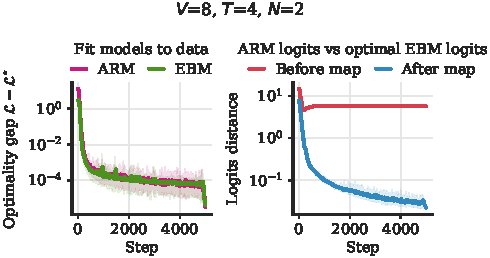
\includegraphics[width=0.6\linewidth]{figures/cvg_and_logits_dist_V8_T4_N2.pdf} 
     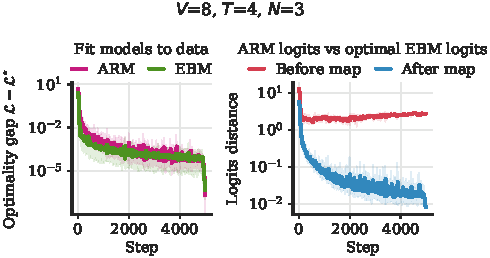
\includegraphics[width=0.6\linewidth]{figures/cvg_and_logits_dist_V8_T4_N3.pdf} 
     \caption{Loss convergence and logits distances for different Transformer sizes.} 
     \label{fig:cvg_logit_dist_N_vary} 
 \end{figure}


\begin{figure} [p]
     \centering 
     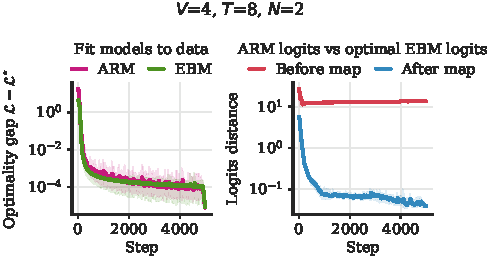
\includegraphics[width=0.6\linewidth]{figures/cvg_and_logits_dist_V4_T8_N2.pdf} 
     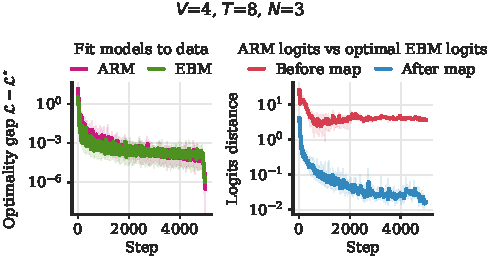
\includegraphics[width=0.6\linewidth]{figures/cvg_and_logits_dist_V4_T8_N3.pdf} 
     \caption{Loss convergence and logits distances for different Transformer sizes in the case  ZXQ0XQZ .} 
     \label{fig:cvg_logit_dist_T_much_gt_V} 
 \end{figure}

\begin{figure} [p]
     \centering 
     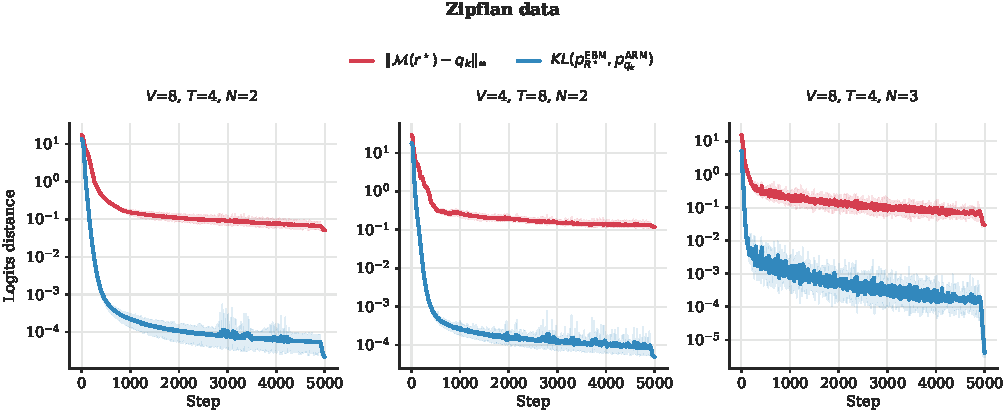
\includegraphics[width=\linewidth]{figures/kl_vs_inf_norm_zipfian.pdf} 
     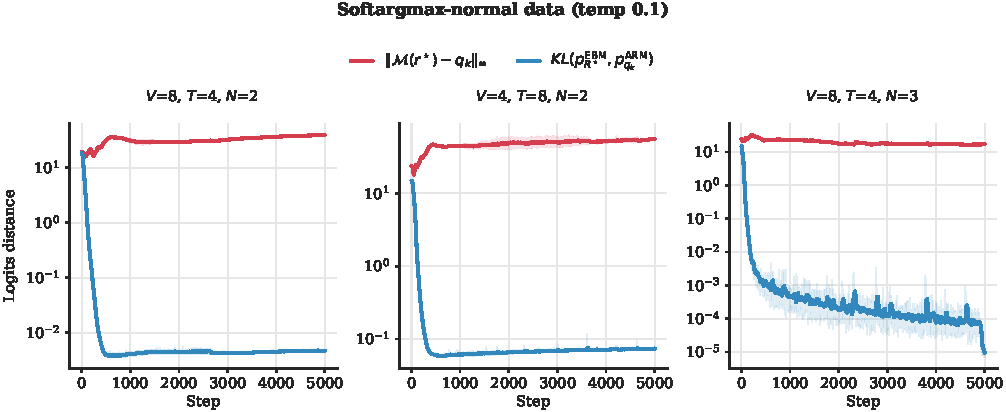
\includegraphics[width=\linewidth]{figures/kl_vs_inf_norm_softmax_normal.pdf} 
     \caption{Comparing KL divergence and logits distance in infinity norm.} 
     \label{fig:kl_vs_inf_norm} 
 \end{figure}

\clearpage

\subsection{Optimization dynamics}

\paragraph{Effect of learning rate.}

이전 실험에서는 학습률이 가장 좋은 결과를 보고했습니다. 그림 \ref{fig:learning_rate_sweep} 및 그림 \ref{fig:training_loss_curves_by_learning_rate}에서는 다양한 학습 속도에 따라 EBM과 ARM을 비교합니다. 이 실험에서 EBM과 ARM은 모두 동일한 학습 속도에서 최적의 성능을 달성하지만 ARM은 학습 속도 사양에 약간 더 강력합니다.

\begin{figure} [h!]
     \centering 
     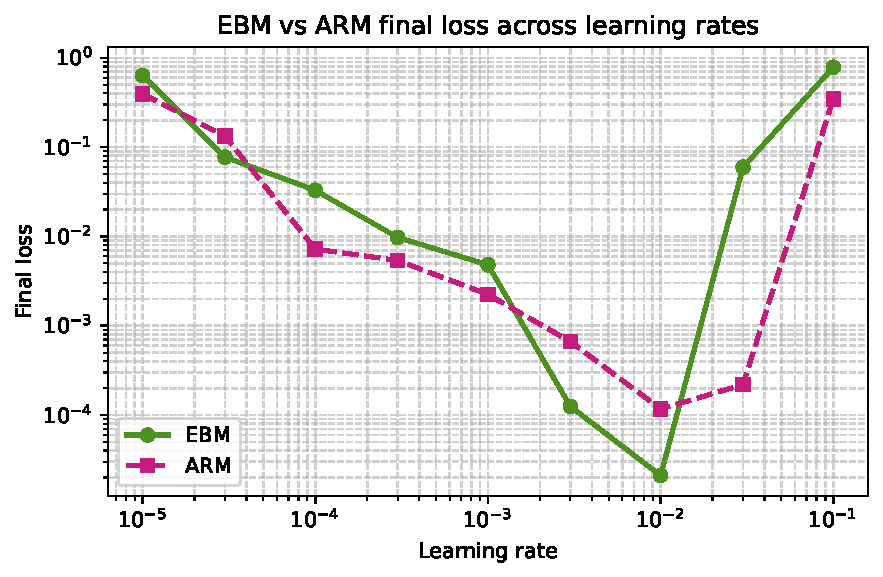
\includegraphics[width=0.50\textwidth]{figures/learning_rate_sweep} 
     \caption{Final loss across learning rates. Both EBMs and ARMs achieve optimal performance at the same learning rate but ARMs are slightly more robust to learning rate specification.} 
     \label{fig:learning_rate_sweep} 
 \end{figure}

\begin{figure} [h!]
     \centering 
     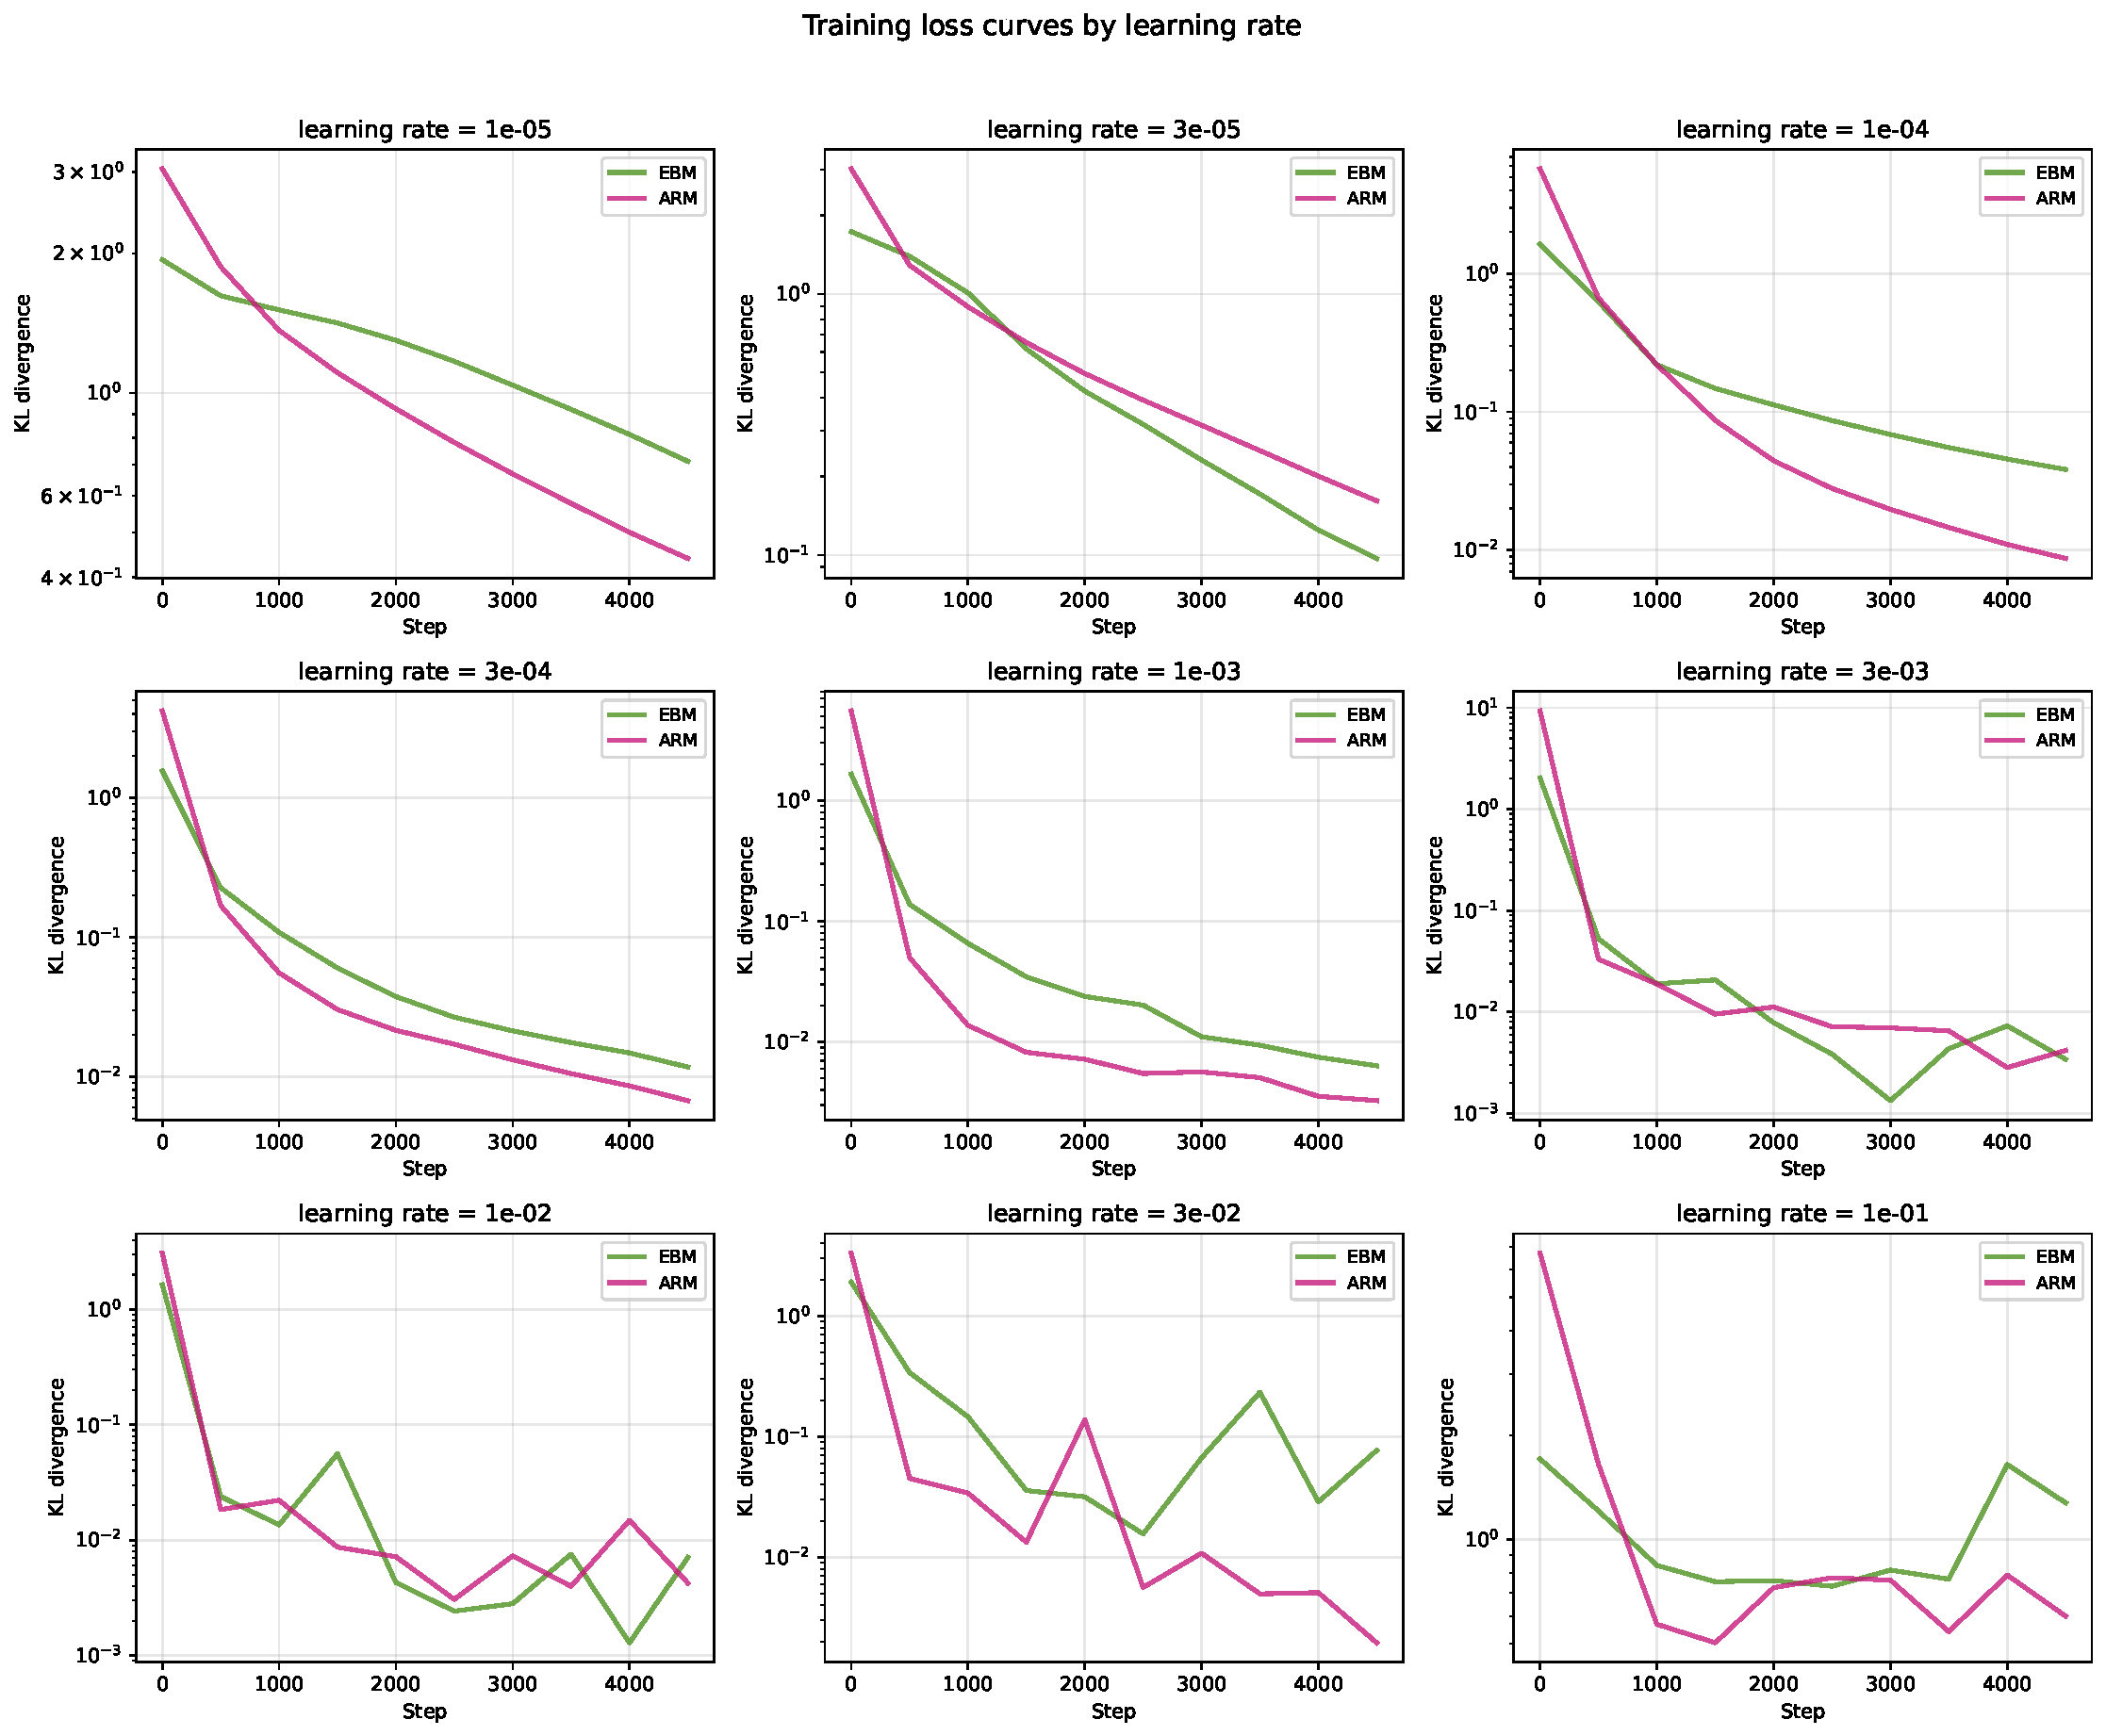
\includegraphics[width=0.75\textwidth]{figures/training_loss_curves_by_learning_rate} 
     \caption{Training loss curves per learning rate. ARMs are more robust to learning rate specification.} 
     \label{fig:training_loss_curves_by_learning_rate} 
 \end{figure}

\paragraph{Gradient noise analysis.}

그림 \ref{fig:gradient_noise}에서는 그래디언트 노이즈 스케일(GNS), 그래디언트 일관성 및 좌표별 신호 대 잡음(SNR) 비율의 세 가지 측정항목을 사용하여 그래디언트 노이즈를 분석했습니다(정의는 캡션 참조). 이 실험에서 EBM과 ARM은 노이즈에 유사하게 민감합니다. 이는 우리 논문의 주요 메시지 중 하나를 다시 한 번 확인시켜 줍니다. 즉, ARM은 EBM과 매우 유사하게 동작할 수 있는 능력이 있습니다(트레이닝 및 샘플링이 훨씬 더 쉽습니다).

\begin{figure}[h!]
     \centering 
     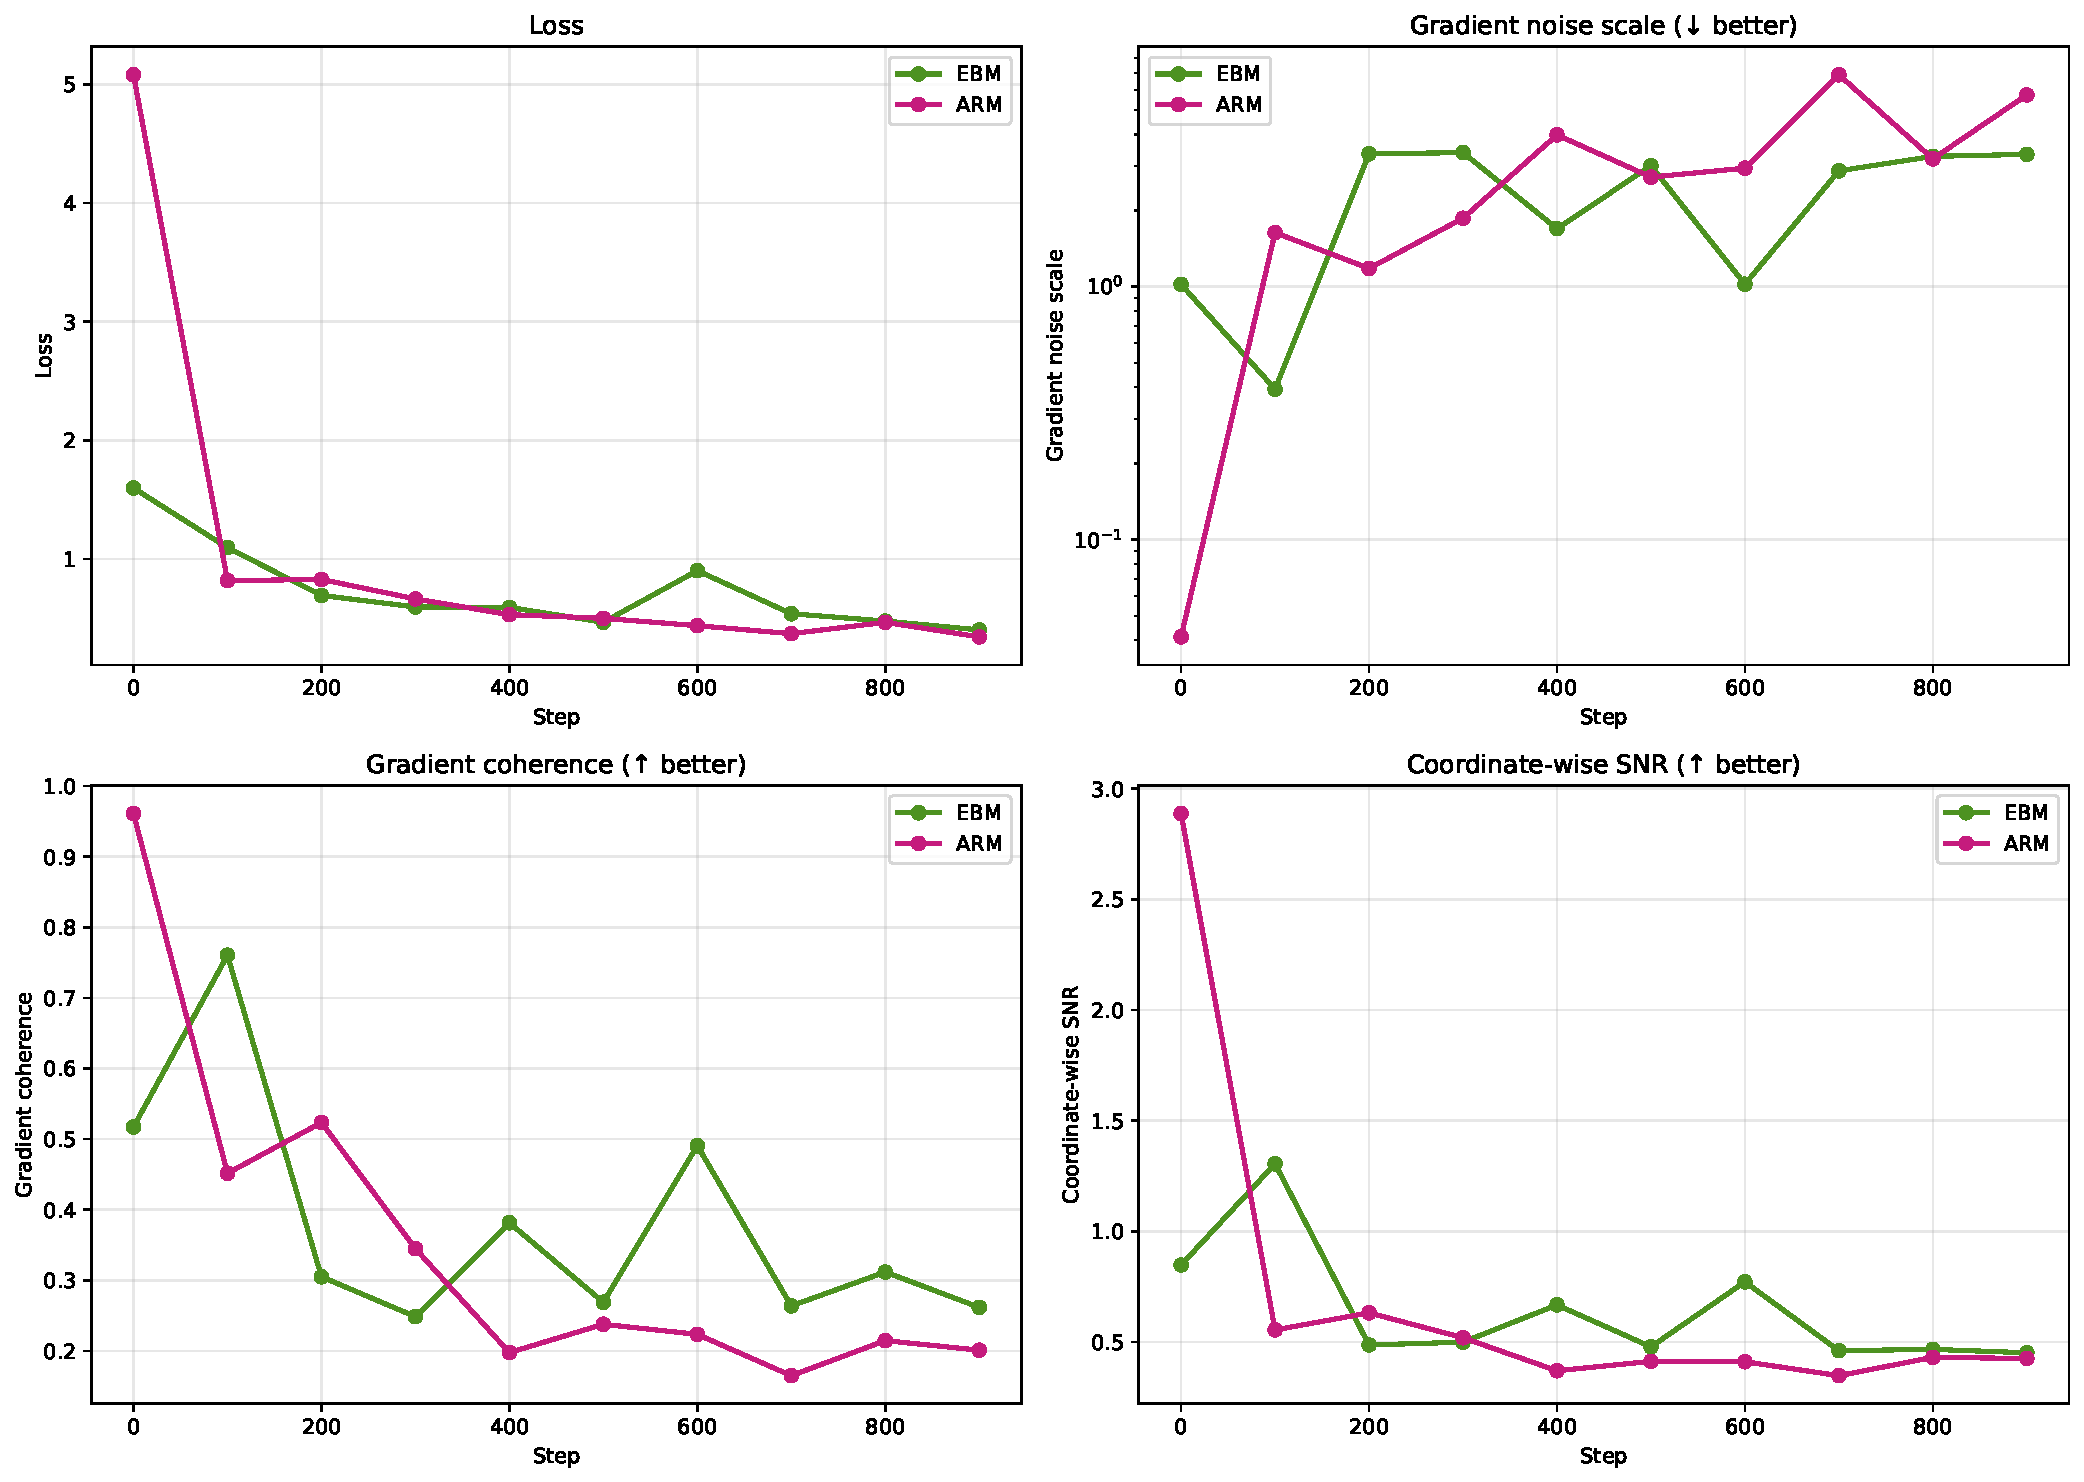
\includegraphics[width=0.95\textwidth]{figures/gradient_noise} 
     \caption{Gradient noise analysis. The three metrics are
     ZXQ0XQZ ,
     ZXQ1XQZ ,
    and  ZXQ2XQZ ,
    where  ZXQ3XQZ  is the mini-batch gradient,
     ZXQ4XQZ , 
     ZXQ5XQZ 
    and  ZXQ6XQZ  is the number of parameters.   
    EBMs and ARMs have similar sensitivity to gradient noise.
    } 
     \label{fig:gradient_noise} 
 \end{figure}

\end{document}
